% ============================================================
% STAT 8289 Course Project - JASA Format
% Title: Performance and Interpretability Trade-offs in
%        Reinforcement Learning for Sepsis Treatment:
%        Comparing Offline and Online Approaches
% Authors: Zhiyu Cheng*, Yalun Ding, Chuanhui Peng (Equal contribution)
%          *Corresponding author: zhiyu.cheng@email.gwu.edu
% Date: October 2025
% ============================================================

\documentclass[11pt]{article}

% ============================================================
% PACKAGES
% ============================================================
\usepackage{amsmath,amssymb}
\usepackage{iftex}
\ifPDFTeX
  \usepackage[T1]{fontenc}
  \usepackage[utf8]{inputenc}
  \usepackage{textcomp}
\else
  \usepackage{unicode-math}
  \defaultfontfeatures{Scale=MatchLowercase}
  \defaultfontfeatures[\rmfamily]{Ligatures=TeX,Scale=1}
\fi
\usepackage{lmodern}

% Formatting
\usepackage{ifthen}
\IfFileExists{microtype.sty}{\usepackage[]{microtype}}{}
\usepackage{xcolor}
\setlength{\emergencystretch}{3em}
\setcounter{secnumdepth}{5}

% Tables and figures
\usepackage{longtable,booktabs,array}
\usepackage{calc}
\usepackage{graphicx}
\usepackage{subcaption}

% Page layout (JASA format)
\addtolength{\oddsidemargin}{-.5in}
\addtolength{\evensidemargin}{-.1in}
\addtolength{\textwidth}{1in}
\addtolength{\textheight}{1.7in}
\addtolength{\topmargin}{-1in}

% Graphics
\makeatletter
\def\maxwidth{\ifdim\Gin@nat@width>\linewidth\linewidth\else\Gin@nat@width\fi}
\def\maxheight{\ifdim\Gin@nat@height>\textheight\textheight\else\Gin@nat@height\fi}
\makeatother
\setkeys{Gin}{width=\maxwidth,height=\maxheight,keepaspectratio}
\makeatletter
\def\fps@figure{htbp}
\makeatother

% Bibliography
\usepackage[]{natbib}
\bibliographystyle{agsm}

% Hyperlinks
\usepackage{bookmark}
\IfFileExists{xurl.sty}{\usepackage{xurl}}{}
\urlstyle{same}
\hypersetup{
  pdftitle={Performance and Interpretability Trade-offs in Reinforcement Learning for Sepsis Treatment: Comparing Offline and Online Approaches},
  pdfauthor={Zhiyu Cheng (corresponding), Yalun Ding, Chuanhui Peng},
  pdfkeywords={Reinforcement Learning, Sepsis Treatment, Interpretability, Conservative Q-Learning, LEG Analysis, Offline RL, MIMIC-III},
  colorlinks=true,
  linkcolor={blue},
  filecolor={red},
  citecolor={blue},
  urlcolor={blue},
  pdfcreator={LaTeX via pandoc}
}

% Custom commands
\newcommand{\anon}{1}  % Set to 0 for anonymous version, 1 for author version

% ============================================================
% DOCUMENT START
% ============================================================
\begin{document}

\def\spacingset#1{\renewcommand{\baselinestretch}{#1}\small\normalsize}
\spacingset{1}

% ============================================================
% TITLE AND AUTHORS
% ============================================================
\if1\anon
{
  \title{\bf Performance and Interpretability Trade-offs in Reinforcement Learning for Sepsis Treatment: Comparing Offline and Online Approaches}
  \author{
    Zhiyu Cheng\thanks{Equal contribution. Authors listed alphabetically. The authors gratefully acknowledge the support of STAT 8289 - Reinforcement Learning course at George Washington University. This work uses the MIMIC-III database (Johnson et al., 2016) and builds upon the gym-sepsis environment (Raghu et al., 2017).}$^{1,*}$,
    Yalun Ding$^{1}$,
    Chuanhui Peng$^{1}$ \\
    $^{1}$Department of Statistics, George Washington University \\
    $^{*}$Corresponding author: zhiyu.cheng@email.gwu.edu
  }
  \maketitle
} \fi

\if0\anon
{
  \bigskip
  \bigskip
  \bigskip
  \begin{center}
    {\LARGE\bf Performance and Interpretability Trade-offs in Reinforcement Learning for Sepsis Treatment: Comparing Offline and Online Approaches}
\end{center}
  \medskip
} \fi

% ============================================================
% ABSTRACT
% ============================================================
\bigskip
\begin{abstract}
Sepsis remains a leading cause of mortality in critical care, and reinforcement learning (RL) offers a promising route to data-driven treatment policies. Yet clinical adoption is impeded by the prevailing assumption that interpretability inevitably compromises performance, and that online RL methods necessarily outperform offline approaches. We interrogate these trade-offs by comparing three offline RL methods (Behavior Cloning, Conservative Q-Learning, and Deep Q-Network trained on static datasets) with three online RL methods (Double DQN with Attention, Double DQN with Residual connections, and Soft Actor-Critic with environment interaction) using the gym-sepsis simulator—a MIMIC-III–derived environment for sepsis treatment. Policy quality is assessed through patient-survival rates stratified by Sequential Organ Failure Assessment (SOFA) states, while interpretability is quantified with Linearly Estimated Gradients (LEG), a model-agnostic feature-importance method.

Across 500 evaluation episodes, online RL achieves marginally higher overall survival (95.4\% for DDQN-Attention vs. 94.2\% for BC), with a 1.9 percentage point advantage on high-severity patients (90.5\% vs. 88.6\%). However, this modest performance gain comes at the cost of requiring extensive environment interaction during training—infeasible in clinical settings where patient safety is paramount. Interpretability analysis reveals that offline methods, particularly CQL, produce LEG saliency peaks of 40.06—roughly 600-fold larger than DQN's 0.069—highlighting clinically coherent emphasis on blood pressure and lactate levels. These results demonstrate that high-performing offline RL policies can deliver comparable survival rates with transparent decision logic and no patient risk during training, challenging the presumed necessity of online learning. Selecting offline algorithms such as CQL therefore offers a viable path toward regulatory-grade, clinician-trustworthy AI for sepsis management.
\end{abstract}

\noindent%
{\it Keywords:} Reinforcement Learning, Sepsis Treatment, Interpretability, Conservative Q-Learning, LEG Analysis, Offline RL, MIMIC-III

\vfill
\newpage
\spacingset{1} % Single line spacing for 25-page limit

% ============================================================
% 1. INTRODUCTION
% ============================================================
% ============================================================
% INTRODUCTION SECTION
% ============================================================

\section{Introduction}\label{sec:intro}

Sepsis remains one of the most pressing challenges in critical care, responsible for nearly twenty percent of global mortality and more than \$62 billion in annual U.S.\ healthcare expenditures \citep{rudd2020sepsis, fleischmann2016sepsis}. Despite successive iterations of the Sepsis-3 definition \citep{singer2016sepsis3} and aggressive early-intervention campaigns, outcomes have plateaued: mortality still ranges from 10--20\% for sepsis without shock to 40--50\% for septic shock. Clinicians must synthesize heterogeneous physiological signals and act within hours, yet existing protocols offer only population-level heuristics for fluid resuscitation, vasopressor titration, and escalation to organ support \citep{rhodes2017ssc}. Large randomized trials that re-evaluated early goal-directed therapy (EGDT) \citep{rivers2001egdt, arise2014} underscore the difficulty of prescribing universally optimal intervention thresholds.

Reinforcement learning (RL) has emerged as a candidate framework for tailoring sepsis therapy to patient trajectories. By optimizing long-horizon rewards, RL-based policies can, in principle, balance competing short-term hemodynamic targets against downstream survival. Early work trained Deep Q-Network (DQN) and fitted Q-iteration policies on MIMIC-III data, showing promising retrospective survival estimates \citep{raghu2017sepsis_drl, komorowski2018ai_clinician}. However, these studies emphasized expected returns and policy deviations from clinician behavior while offering only qualitative or aggregate descriptions of why certain actions were recommended. As sepsis RL research shifts toward the offline setting—where algorithms must learn exclusively from historical data—questions about policy interpretability become central. Offline methods ranging from Behavior Cloning (BC) to Conservative Q-Learning (CQL) and offline-adapted DQN handle uncertainty and distribution shift differently, which plausibly shapes the transparency of their learned decision rules.

A rigorous understanding of how offline RL algorithms trade off performance and interpretability is still missing. Existing evaluations lack quantitative feature-attribution analyses—a gap with direct regulatory consequences. The U.S.\ Food and Drug Administration requires explainable AI systems for medical decision support \citep{fda2021ai}, yet no sepsis RL study has demonstrated whether high-performing policies expose clinically plausible decision rationales that clinicians can validate and trust \citep{holzinger2017xai_healthcare}. Moreover, interpretability techniques for sequential decision-making—such as Linearly Estimated Gradients (LEG) saliency maps \citep{greydanus2018leg}—have rarely been applied to healthcare RL, so it remains unclear which algorithmic choices yield explanations aligned with accepted sepsis physiology.

Responding to this gap, we ask: \textit{Can offline RL algorithms for sepsis simultaneously deliver state-of-the-art survival performance and clinically interpretable decision rationales?} We hypothesize that performance--interpretability trade-offs depend on algorithmic design and that conservatism in the objective (as in CQL) can enhance both safety and transparency. To test this hypothesis, we train BC, CQL, and DQN policies on a dataset of simulated patient trajectories generated by rolling out a heuristic policy in the gym-sepsis simulator—an environment whose dynamics and outcome models were trained on MIMIC-III data \citep{raghu2017sepsis_drl}. We jointly evaluate survival outcomes stratified by Sequential Organ Failure Assessment (SOFA) scores and LEG-based feature saliency, ensuring that both performance and interpretability are quantified rigorously.

This study contributes (i) the first quantitative benchmark of offline RL algorithms on both outcome metrics and interpretability for sepsis management, (ii) empirical evidence that the presumed performance--interpretability tension is not inevitable, with CQL matching the survival of alternative policies while providing salient, guideline-consistent explanations, and (iii) methodological guidance on applying LEG analysis to safety-critical RL deployments. Section~\ref{sec:related} surveys clinical RL and interpretability research, Section~\ref{sec:problem} formalizes the sepsis decision process and LEG framework, Section~\ref{sec:methods} details experimental design, Section~\ref{sec:results} reports performance and interpretability findings, Section~\ref{sec:discussion} interprets the implications for clinical adoption, and Section~\ref{sec:conclusion} outlines future research directions.

% End of Introduction section



% ============================================================
% 2. RELATED WORK
% ============================================================
% ============================================================
% RELATED WORK SECTION
% ============================================================

\section{Related Work}\label{sec:related}

Our work builds on three research areas: reinforcement learning for sepsis treatment, offline RL algorithms, and interpretability methods for RL policies.

% ============================================================
\subsection{Reinforcement Learning for Sepsis Treatment}\label{sec:related:sepsis}

Raghu et al. \citeyearpar{raghu2017sepsis_drl} pioneered deep RL for sepsis treatment using the MIMIC-III database, formulating treatment as a discrete-action MDP with a $5 \times 5$ action grid (IV fluid × vasopressor dosing). Their work established the gym-sepsis simulation environment we use in this study. Komorowski et al. \citeyearpar{komorowski2018ai_clinician} developed the AI Clinician using fitted Q-iteration, achieving 98\% survival in retrospective simulation. While these studies demonstrated high performance, \textbf{neither provided quantitative feature-attribution analysis}. Their interpretability assessments relied on visualizing aggregate action distributions, revealing \textit{what} the policy does but not \textit{why}—a critical gap for regulatory approval and clinical trust. Recent work by Yao et al. \citeyearpar{yao2021sepsis_cql} applied CQL to sepsis but did not evaluate policy interpretability systematically.


% ============================================================
\subsection{Offline Reinforcement Learning}\label{sec:related:offline}

Offline RL learns from fixed datasets without environment interaction, addressing distributional shift when learned policies select out-of-distribution (OOD) actions \citep{levine2020offline}. \textbf{Behavior Cloning (BC)} \citep{pomerleau1991bc} treats offline RL as supervised imitation learning, avoiding distributional shift but cannot improve beyond the behavioral policy. \textbf{Conservative Q-Learning (CQL)} \citep{kumar2020cql} adds a conservatism penalty that discourages high Q-values for OOD actions, providing safety guarantees for healthcare. CQL's penalty encourages simpler Q-function representations aligned with the behavioral policy—when the behavioral policy follows interpretable threshold rules, CQL may learn Q-functions with strong gradients detectable by saliency analysis. \textbf{Deep Q-Network (DQN)} \citep{mnih2015dqn} combines Q-learning with deep networks and experience replay; originally designed for online learning, it can be adapted to offline settings but tends to overestimate OOD action values.


% ============================================================
\subsection{Interpretability Methods in RL}\label{sec:related:interp}

Regulatory agencies require explainable AI for medical decision support \citep{holzinger2017xai_healthcare}, yet deep RL policies are notoriously opaque. Greydanus et al. \citeyearpar{greydanus2018leg} introduced \textbf{Linearly Estimated Gradients (LEG)}, a perturbation-based method that approximates Q-function gradients via local linear regression, producing saliency maps highlighting which features drive action selection. We adopt LEG because it is model-agnostic (enabling fair comparison across algorithms), produces quantitative saliency scores, and aligns with clinical intuition where clinicians weight physiological indicators. No prior healthcare RL work has systematically compared interpretability across algorithms using gradient-based methods.


% ============================================================
\subsection{Research Gap}\label{sec:related:gap}

Despite a decade of sepsis RL research achieving strong retrospective performance, quantitative interpretability evaluation remains absent. While offline RL methods differ fundamentally in handling distributional shift, no study has examined whether these algorithmic differences translate to interpretability differences. Our work addresses this gap by jointly benchmarking offline and online RL on both survival outcomes and LEG-based interpretability, providing the first quantitative evidence on the performance--interpretability trade-off across RL paradigms.

% End of Related Work section


% ============================================================
% 3. PROBLEM FORMULATION
% ============================================================
% ============================================================
% PROBLEM FORMULATION SECTION
% ============================================================

\section{Problem Formulation}\label{sec:problem}

We formulate sepsis treatment as a finite-horizon Markov Decision Process (MDP) in the offline reinforcement learning setting, where the goal is to learn an optimal policy from a fixed dataset without further environment interaction. We define interpretability through the Linearly Estimated Gradients (LEG) framework for quantitative feature importance measurement.

% ============================================================
\subsection{MDP Formulation}\label{sec:problem:mdp}

The sepsis treatment MDP is defined by the tuple $\mathcal{M} = (\mathcal{S}, \mathcal{A}, \mathcal{P}, \mathcal{R}, \gamma)$. The \textbf{state space} $\mathcal{S} \subset \mathbb{R}^{46}$ captures patient physiological condition through laboratory values, vital signs, and clinical severity scores as detailed in Section~\ref{sec:methods:env}. The \textbf{action space} $\mathcal{A}$ contains 25 discrete actions representing a $5 \times 5$ grid of IV fluid and vasopressor dosing levels. The \textbf{transition dynamics} $\mathcal{P}(s_{t+1} | s_t, a_t)$ are learned from MIMIC-III data via the gym-sepsis simulator \citep{raghu2017sepsis_drl}. The \textbf{reward function} uses sparse terminal rewards: $\mathcal{R}(s_T, a_T) = +15$ for survival, $-15$ for death, and $0$ for intermediate steps. We use discount factor $\gamma = 0.99$.

A policy $\pi: \mathcal{S} \to \Delta(\mathcal{A})$ maps states to action distributions. The goal is to find $\pi^* = \arg\max_\pi V^\pi(s)$ where the value function is:
\begin{equation}
V^\pi(s) = \mathbb{E}_{\tau \sim \pi, \mathcal{P}} \left[ \sum_{t=0}^{H-1} \gamma^t \mathcal{R}(s_t, a_t) \,\Big|\, s_0 = s \right].
\end{equation}
The action-value function $Q^\pi(s, a)$ represents expected return when taking action $a$ in state $s$ and following $\pi$ thereafter. The optimal policy is derived via $\pi^*(s) = \arg\max_a Q^*(s, a)$.


% ============================================================
\subsection{Offline RL Setting}\label{sec:problem:offline}

In offline RL, the agent learns exclusively from a fixed dataset $\mathcal{D} = \{(s_i, a_i, r_i, s'_i)\}_{i=1}^N$ collected under a behavioral policy, without environment interaction during training \citep{levine2020offline}. The central challenge is \textit{distributional shift}: the learned policy $\pi$ may select out-of-distribution (OOD) actions where Q-value estimates are unreliable due to extrapolation error \citep{fujimoto2019offpolicy}.

Conservative Q-Learning (CQL) \citep{kumar2020cql} addresses this via pessimism, penalizing Q-values for OOD actions:
\begin{equation}
\min_Q \, \mathbb{E}_{(s,a,r,s') \sim \mathcal{D}} \left[ \left( Q(s, a) - \left( r + \gamma \max_{a'} Q(s', a') \right) \right)^2 \right] + \alpha \cdot \mathbb{E}_{s \sim \mathcal{D}} \left[ \log \sum_{a} \exp(Q(s, a)) - \mathbb{E}_{a \sim \pi_{\text{behav}}} [Q(s, a)] \right],
\end{equation}
where $\alpha > 0$ controls conservatism strength. Behavior Cloning (BC) avoids distributional shift by imitating the behavioral policy via supervised learning: $\pi_{\text{BC}} = \arg\max_\pi \mathbb{E}_{(s, a) \sim \mathcal{D}} [\log \pi(a | s)]$, but cannot improve beyond the behavioral policy's performance.


% ============================================================
\subsection{Interpretability via LEG}\label{sec:problem:interp}

Interpretability quantifies the extent to which clinicians can understand policy decisions—critical for regulatory approval \citep{fda2021ai} and clinical trust \citep{holzinger2017xai_healthcare}. We use Linearly Estimated Gradients (LEG) \citep{greydanus2018leg}, a model-agnostic perturbation method measuring feature importance.

For a policy $\pi$ and state $s$, LEG approximates the saliency (gradient) of the Q-function with respect to each state feature via:
\begin{enumerate}
\item Sample $M = 1000$ perturbations $\delta^{(m)} \sim \mathcal{N}(0, \sigma^2 I)$ with $\sigma = 0.05$
\item Evaluate perturbed Q-values: $\Delta Q^{(m)} = Q(s + \delta^{(m)}, a) - Q(s, a)$
\item Fit linear regression: $\Delta Q^{(m)} \approx \sum_{j=1}^{46} w_j \cdot \delta_j^{(m)}$ via OLS
\item Extract saliency scores: $\text{Saliency}_j(s, a) = w_j$
\end{enumerate}

We quantify interpretability via: (1) \textbf{maximum saliency magnitude} $\max_{s, j} |\text{Saliency}_j(s, a)|$, measuring signal strength; (2) \textbf{saliency range}, capturing feature differentiation; (3) \textbf{clinical coherence}, assessing whether top features align with medical knowledge (e.g., blood pressure, lactate for sepsis). Policies with strong saliency signals ($>10$), large ranges, and high clinical coherence are deemed interpretable.

% End of Problem Formulation section


% ============================================================
% 4. METHODS
% ============================================================
% ============================================================
% METHODS SECTION
% ============================================================

\section{Methods}\label{sec:methods}

We describe the experimental setup: the gym-sepsis simulation environment, offline and online RL algorithms, LEG interpretability analysis, and evaluation protocol.

% ============================================================
\subsection{Environment and Data}\label{sec:methods:env}

\subsubsection{Gym-Sepsis Simulator}

We use Gym-Sepsis \citep{raghu2017sepsis_drl}, an RL simulator for ICU sepsis treatment trained on MIMIC-III data \citep{johnson2016mimic3}.

\textbf{State Space.} At each timestep, the state is a 46-dimensional vector spanning laboratory values (lactate, creatinine, platelet count, etc.), vital signs (blood pressure, heart rate, SpO$_2$, etc.), demographics (age, gender, race), clinical severity scores (SOFA, LODS, SIRS, qSOFA, Elixhauser), and treatment status (mechanical ventilation, blood culture). The SOFA score \citep{vincent1996sofa} ranges from 0--24, with higher values indicating greater organ dysfunction; we use SOFA for severity stratification in Section~\ref{sec:methods:eval}.

\textbf{Action Space.} A discrete $5 \times 5$ grid over IV fluid and vasopressor dosage bins (action $ = 5 \times \text{IV\_bin} + \text{VP\_bin}$), yielding 25 actions.

\textbf{Episode Dynamics \& Reward.} Episodes span ICU stays (4-hour timesteps) until discharge or death. Sparse reward: $r_t = +15$ (survival), $-15$ (death), $0$ (intermediate).

\subsubsection{Offline Training Dataset}

We generated an offline dataset of 10,000 episodes (~100K transitions) using a heuristic policy based on clinical guidelines \citep{rhodes2017ssc, seymour2017sepsis_criteria}, achieving 94.6\% survival. Data partitioning: 9,000 train, 500 validation, 500 test episodes.

% ============================================================
\subsection{Algorithms}\label{sec:methods:algos}

We compare three offline RL algorithms representing different learning paradigms: Behavior Cloning (supervised learning), Conservative Q-Learning (offline Q-learning), and Deep Q-Network (online RL adapted for offline evaluation). All algorithms use the same neural network architecture for fair comparison: a 3-layer multilayer perceptron (MLP) with hidden dimensions [256, 256, 128] and ReLU activations.

\subsubsection{Behavior Cloning (BC)}

Behavior Cloning treats offline RL as a supervised learning problem, training a policy to imitate the behavioral policy by minimizing the negative log-likelihood of observed actions \citep{pomerleau1991bc}. Formally, given a dataset $\mathcal{D} = \{(s_i, a_i)\}_{i=1}^N$ of state-action pairs, BC learns a policy $\pi_{\theta}(a|s)$ by solving:
\begin{equation}
\theta^* = \arg\min_{\theta} -\frac{1}{N} \sum_{i=1}^N \log \pi_{\theta}(a_i | s_i)
\end{equation}

BC is computationally efficient and stable, but suffers from distribution shift when the learned policy encounters states not well-represented in the offline dataset \citep{ross2010dagger}.

\textbf{Implementation.} We use d3rlpy's DiscreteBCConfig with batch size 1,024, learning rate $1 \times 10^{-3}$ (Adam), training for 50,000 gradient steps (10 epochs $\times$ 5,000 steps/epoch).

\subsubsection{Conservative Q-Learning (CQL)}

Conservative Q-Learning \citep{kumar2020cql} is an offline RL algorithm that learns a conservative Q-function to avoid overestimation on out-of-distribution actions. CQL augments the standard Bellman error with a conservatism penalty that pushes down Q-values for unseen actions while pushing up Q-values for actions in the dataset:
\begin{equation}
\min_Q \alpha \cdot \mathbb{E}_{s \sim \mathcal{D}} \left[ \log \sum_a \exp Q(s, a) - \mathbb{E}_{a \sim \pi_\beta} Q(s, a) \right] + \frac{1}{2} \mathbb{E}_{(s,a,r,s') \sim \mathcal{D}} \left[ (Q(s,a) - \mathcal{T}^\pi Q(s,a))^2 \right]
\end{equation}
where $\alpha$ controls the strength of the conservatism penalty, $\pi_\beta$ is the behavioral policy, and $\mathcal{T}^\pi$ is the Bellman operator.

The conservatism penalty encourages the learned Q-function to assign lower values to actions that were not taken by the behavioral policy, reducing the risk of selecting suboptimal actions due to Q-value overestimation. The policy is derived as $\pi(s) = \arg\max_a Q(s, a)$.

\textbf{Implementation.} We use d3rlpy's DiscreteCQLConfig with batch size 1,024, learning rate $3 \times 10^{-4}$ (Adam), $\alpha = 1.0$, target network updates every 2,000 steps, training for 200,000 gradient steps.

\subsubsection{Deep Q-Network (DQN)}

Deep Q-Network \citep{mnih2015dqn} is a foundational deep RL algorithm that combines Q-learning with deep neural networks. DQN uses two key techniques for stability: (1) experience replay, which stores transitions in a replay buffer and samples mini-batches for training, and (2) a target network $Q_{\theta^-}$ that is periodically synchronized with the main network $Q_\theta$ to stabilize Q-value targets.

The Q-function is updated to minimize the temporal difference (TD) error:
\begin{equation}
\mathcal{L}(\theta) = \mathbb{E}_{(s,a,r,s') \sim \mathcal{D}} \left[ \left( Q_\theta(s,a) - \left( r + \gamma \max_{a'} Q_{\theta^-}(s', a') \right) \right)^2 \right]
\end{equation}

The policy is derived greedily as $\pi(s) = \arg\max_a Q_\theta(s, a)$, with $\epsilon$-greedy exploration during training ($\epsilon$ annealed from 1.0 to 0.05).

\textbf{Implementation and Training Paradigm.} We use the Stable-Baselines3 library for DQN training. Unlike BC and CQL, which are designed explicitly for offline learning from a fixed dataset, DQN was trained \textit{online} by interacting with the Gym-Sepsis simulator and accumulating experience in a replay buffer of size 100,000. This methodological choice reflects DQN's original design as an online RL algorithm \citep{mnih2015dqn} and enables us to compare interpretability across both offline-specific methods (BC, CQL) and online methods adapted for safety-critical domains. We label our study as focusing on "offline RL" because BC and CQL are trained offline, and \textit{all three algorithms are evaluated identically in offline mode}—i.e., policies are tested on a held-out set of 500 episodes without further environment interaction. This evaluation protocol ensures fair comparison: DQN's online training provides it with potentially richer exploration data, yet it must still generalize to unseen test episodes in the same manner as offline-trained policies. Thus, our interpretability analysis reflects how each algorithm's learned representations (whether from offline or online training) manifest in deployment settings where no further learning occurs.

DQN uses batch size 256, learning rate $1 \times 10^{-4}$ (Adam), target network updates every 1,000 steps, $\epsilon$-greedy exploration (1.0 $\to$ 0.05), training for 100,000 timesteps.

\subsubsection{Online RL Algorithms}\label{sec:methods:algos:online}

To provide a comprehensive comparison between offline and online RL paradigms, we also evaluate three state-of-the-art online RL algorithms with architectural innovations (implemented by collaborator Y. Ding). Unlike the offline methods above, these algorithms train by interacting with the Gym-Sepsis simulator, collecting 1 million timesteps of experience through exploration. This comparison illuminates the performance-safety trade-off: online methods can explore beyond the behavioral policy's distribution but require environment access during training—a significant constraint in clinical settings where patient safety prohibits trial-and-error learning.

\paragraph{Double DQN with Attention (DDQN-Attention).}
This algorithm extends Double DQN \citep{vanHasselt2016double_dqn} with a multi-head self-attention mechanism in the encoder network. Double DQN addresses Q-value overestimation by decoupling action selection and evaluation: the main network selects the best action, while the target network evaluates it. The attention layer allows the model to dynamically weight different state features based on their relevance to the current decision:
\begin{equation}
h_t = \text{MultiHeadAttention}(s_t, s_t, s_t) + s_t
\end{equation}
where the residual connection helps gradient flow during backpropagation. The attention mechanism computes scaled dot-product attention across 4 parallel heads, each learning different feature correlations. The encoder uses two hidden layers of 256 and 128 units respectively, with the attention layer inserted after the first hidden layer to capture high-level feature interactions.

\paragraph{Double DQN with Residual Connections (DDQN-Residual).}
This variant incorporates deep residual networks \citep{he2016deep} to enable training of deeper Q-networks without gradient vanishing. The architecture uses three hidden layers of 256 units each, with skip connections between layers:
\begin{equation}
h_{l+1} = \sigma(\text{LayerNorm}(W_l h_l + b_l + h_l))
\end{equation}
where $\sigma$ is the ReLU activation, $W_l$ and $b_l$ are learnable weights and biases, and the additive skip connection $h_l$ preserves gradient information. Layer normalization stabilizes training by normalizing activations within each layer. The residual architecture is hypothesized to learn more complex value functions by decomposing Q-value estimation into a base value plus incremental adjustments.

\paragraph{Soft Actor-Critic (SAC).}
SAC \citep{haarnoja2018soft} is a maximum entropy RL algorithm that optimizes both expected return and policy entropy, encouraging exploration and robustness. The objective function is:
\begin{equation}
J(\pi) = \mathbb{E}_{\tau \sim \pi}\left[\sum_t r(s_t, a_t) + \alpha \mathcal{H}(\pi(\cdot|s_t))\right]
\end{equation}
where $\mathcal{H}(\pi(\cdot|s))$ is the entropy of the policy at state $s$, and $\alpha$ is a temperature parameter that balances exploitation (maximizing reward) and exploration (maximizing entropy). We use the discrete action space variant of SAC with a residual encoder architecture (3 layers of 256 units with skip connections). The temperature $\alpha$ is automatically tuned during training using a dual gradient descent approach \citep{haarnoja2018soft_applications}, starting from $\alpha = 0.2$ and adjusting to maintain a target entropy equal to 95\% of the maximum entropy $\log(25)$ for the 25-action space.

\paragraph{Training Details.}
All three online RL algorithms were trained with 1,000,000 environment interaction steps using experience replay buffers of size 100,000. Training used batch size 256, learning rate $3 \times 10^{-4}$ (Adam), and target network soft updates with $\tau = 0.005$. Exploration for DDQN variants used $\epsilon$-greedy with $\epsilon$ annealed from 1.0 to 0.05 over the first 100,000 steps. Unlike offline methods which require only the pre-collected dataset, these algorithms necessitate access to the simulator during training—a key distinction when considering deployment in clinical settings where patient safety prohibits exploratory interventions.

% ============================================================
\subsection{LEG Interpretability Analysis}\label{sec:methods:leg}

To assess interpretability, we employ Linearly Estimated Gradients (LEG) \citep{greydanus2018leg}, a model-agnostic perturbation-based method for computing feature importance in RL policies. LEG approximates the gradient $\nabla_s Q(s_0, \pi(s_0))$ by sampling perturbations around a given state and performing ridge regression on Q-value changes to obtain saliency scores $\hat{\gamma}_j$ for each feature $j$. We apply LEG to all algorithms using 1,000 perturbation samples per state, analyzing 10 representative states sampled uniformly across SOFA severity levels. We quantify interpretability using three metrics: maximum saliency magnitude (strength of strongest feature signal), saliency range (spread of importance across features), and clinical coherence (alignment with medical knowledge). Full mathematical formulation and implementation details are provided in Appendix~\ref{appendix:leg}.

% ============================================================
\subsection{Evaluation Metrics}\label{sec:methods:eval}

We evaluate algorithm performance using the following metrics:

\subsubsection{Primary Outcome Metrics}

\textbf{Survival rate} (proportion of episodes ending in discharge), \textbf{average return} ($\bar{R} = \frac{1}{N} \sum_i \sum_t r_{i,t}$), and \textbf{average episode length}.

\subsubsection{SOFA-Stratified Analysis}

Episodes stratified by SOFA score: \textbf{low} ($\leq$5), \textbf{medium} (6-10), \textbf{high} ($\geq$11), reporting survival rate per stratum.

\subsubsection{Statistical Significance Testing}

We assess statistical significance of survival rate differences using a chi-square test for categorical outcomes across algorithms. Confidence intervals for survival rates are computed using the Wilson score interval with 95\% confidence level.

% ============================================================
\subsection{Baseline Policies}\label{sec:methods:baselines}

To contextualize RL algorithm performance, we evaluate two baseline policies:

\subsubsection{Random Policy}

The random policy selects actions uniformly at random from the 25-action space at each timestep, i.e., $\pi(a|s) = \frac{1}{25}$ for all $s, a$. This provides a lower bound on expected performance and tests the difficulty of the environment.

\subsubsection{Heuristic Policy}

Implements threshold-based rules from sepsis guidelines \citep{rhodes2017ssc}: escalate IV fluids when SysBP$<$100 mmHg or lactate$>$2.0 mmol/L; escalate vasopressors when MeanBP$<$65 mmHg. Achieved 94.6\% survival.

\subsubsection{Evaluation Protocol}

All policies (random, heuristic, BC, CQL, DQN) are evaluated on 500 episodes in the Gym-Sepsis simulator using identical random seeds for reproducibility. Each episode is initialized with a random patient state sampled from the MIMIC-III-derived distribution. Policies are evaluated deterministically (no exploration noise) to assess their learned behavior.

% End of Methods section



% ============================================================
% 5. RESULTS
% ============================================================
% ============================================================
% RESULTS SECTION
% ============================================================

\section{Results}\label{sec:results}

We present the evaluation results for all policies across 500 episodes each, focusing on overall performance, SOFA-stratified analysis, and most importantly, the LEG interpretability comparison that reveals dramatic differences in feature importance patterns across algorithms.

% ============================================================
\subsection{Overall Performance Comparison}\label{sec:results:overall}

Table \ref{tab:overall-performance} and Figure \ref{fig:algorithm-comparison} summarize the performance of all eight policies evaluated in this study: two baselines (random and heuristic), three offline RL algorithms (BC, CQL, DQN), and three online RL algorithms (DDQN-Attention, DDQN-Residual, SAC). Among all methods, DDQN-Attention achieves the highest survival rate at 95.4\%, demonstrating the benefit of attention mechanisms for feature selection in complex medical domains. SAC achieves 94.8\% survival, while DDQN-Residual achieves 94.2\%, comparable to BC (94.2\%). The random and heuristic baselines achieve 95.0\% and 94.6\% respectively, demonstrating that simple threshold-based clinical rules are remarkably effective in this simulation environment. All methods fall within a narrow 1.4 percentage point range (94.0--95.4\%), with online RL methods achieving marginally higher survival rates than offline RL (95.4\%, 94.8\%, 94.2\% vs. 94.2\%, 94.0\%, 94.0\%).

\textbf{Random Policy Paradox.} The counterintuitive finding that random action selection achieves the highest survival rate (95.0\%) warrants explanation. This result likely reflects an artifact of the Gym-Sepsis simulator's dynamics rather than a substantive finding about sepsis treatment. The simulator, trained on MIMIC-III data, may have learned a relatively forgiving outcome model where patient survival is robust to treatment variation, particularly when treatment actions remain within reasonable ranges (as random selection from the 25-action grid ensures). Additionally, the sparse reward structure provides no intermediate feedback to penalize suboptimal actions during treatment, allowing even poorly targeted interventions to succeed if they avoid extreme under-treatment or over-treatment. This high baseline survival rate ($\sim$94--95\% across all policies) underscores the limitations of using simulator-only evaluation and highlights the need for real-world validation where treatment quality more decisively affects outcomes.

Average cumulative returns mirror the survival rate patterns: DDQN-Attention achieves the highest return at 13.62 $\pm$ 6.28, followed by SAC at 13.44 $\pm$ 6.66, random at 13.50 $\pm$ 6.54, and heuristic at 13.38 $\pm$ 6.78. Offline RL methods achieve slightly lower returns: BC at 13.26 $\pm$ 7.01, CQL and DQN both at 13.20 $\pm$ 7.12. The high standard deviations reflect the sparse reward structure, where episodes yield either +15 (survival) or -15 (death) with minimal intermediate rewards. Average episode lengths vary from 7.7 timesteps (SAC) to 9.5 timesteps (BC, CQL, heuristic), with online RL methods generally achieving shorter episodes (7.7--9.0) compared to offline methods (7.8--9.5). The shorter episode lengths for online RL and offline DQN suggest that these algorithms may have learned more aggressive treatment strategies that accelerate patient discharge, though this does not translate to substantially improved survival outcomes.

However, this modest performance gain for online RL (1.2--1.4 percentage points over the best offline method) comes at a significant practical cost: online methods require extensive environment interaction during training (1 million timesteps)—infeasible in clinical settings where patient safety prohibits trial-and-error learning. In contrast, offline RL methods achieve comparable survival rates (94.0--94.2\%) using only pre-collected data, with no patient risk during training. This small performance gap, combined with the safety constraints of clinical deployment, motivates our focus on interpretability as a critical secondary criterion for algorithm selection. As we will demonstrate in Section~\ref{sec:results:leg}, offline methods—particularly CQL—offer superior interpretability without sacrificing performance, making them more suitable for clinical decision support systems.

\begin{table}[htbp]
\centering
\caption{Overall performance comparison across baseline and RL policies over 500 evaluation episodes. All methods achieve similar overall survival rates (94.0--95.4\%). Online RL methods (DDQN-Attention, DDQN-Residual, SAC) achieve marginally higher survival rates, with DDQN-Attention reaching the highest at 95.4\%, but this comes at the cost of requiring environment interaction during training.}
\label{tab:overall-performance}
\begin{tabular}{lcccc}
\toprule
\textbf{Model} & \textbf{Survival (\%)} & \textbf{Avg Return} & \textbf{Avg Length} & \textbf{Paradigm} \\
\midrule
\multicolumn{5}{l}{\textit{Baselines}} \\
Random          & 95.0               & 13.50 $\pm$ 6.54    & 9.3 $\pm$ 1.1       & -- \\
Heuristic       & 94.6               & 13.38 $\pm$ 6.78    & 9.5 $\pm$ 1.2       & -- \\
\midrule
\multicolumn{5}{l}{\textit{Offline RL}} \\
BC              & 94.2               & 13.26 $\pm$ 7.01    & 9.5 $\pm$ 0.6       & Offline \\
CQL             & 94.0               & 13.20 $\pm$ 7.12    & 9.5 $\pm$ 0.5       & Offline \\
DQN             & 94.0               & 13.20 $\pm$ 7.12    & 7.8 $\pm$ 1.2       & Offline \\
\midrule
\multicolumn{5}{l}{\textit{Online RL}} \\
DDQN-Attention  & \textbf{95.4}      & 13.62 $\pm$ 6.28    & 7.9 $\pm$ 1.0       & Online \\
DDQN-Residual   & 94.2               & 13.26 $\pm$ 7.01    & 9.0 $\pm$ 0.8       & Online \\
SAC             & 94.8               & 13.44 $\pm$ 6.66    & 7.7 $\pm$ 1.2       & Online \\
\bottomrule
\end{tabular}
\end{table}

\begin{figure}[htbp]
\centering
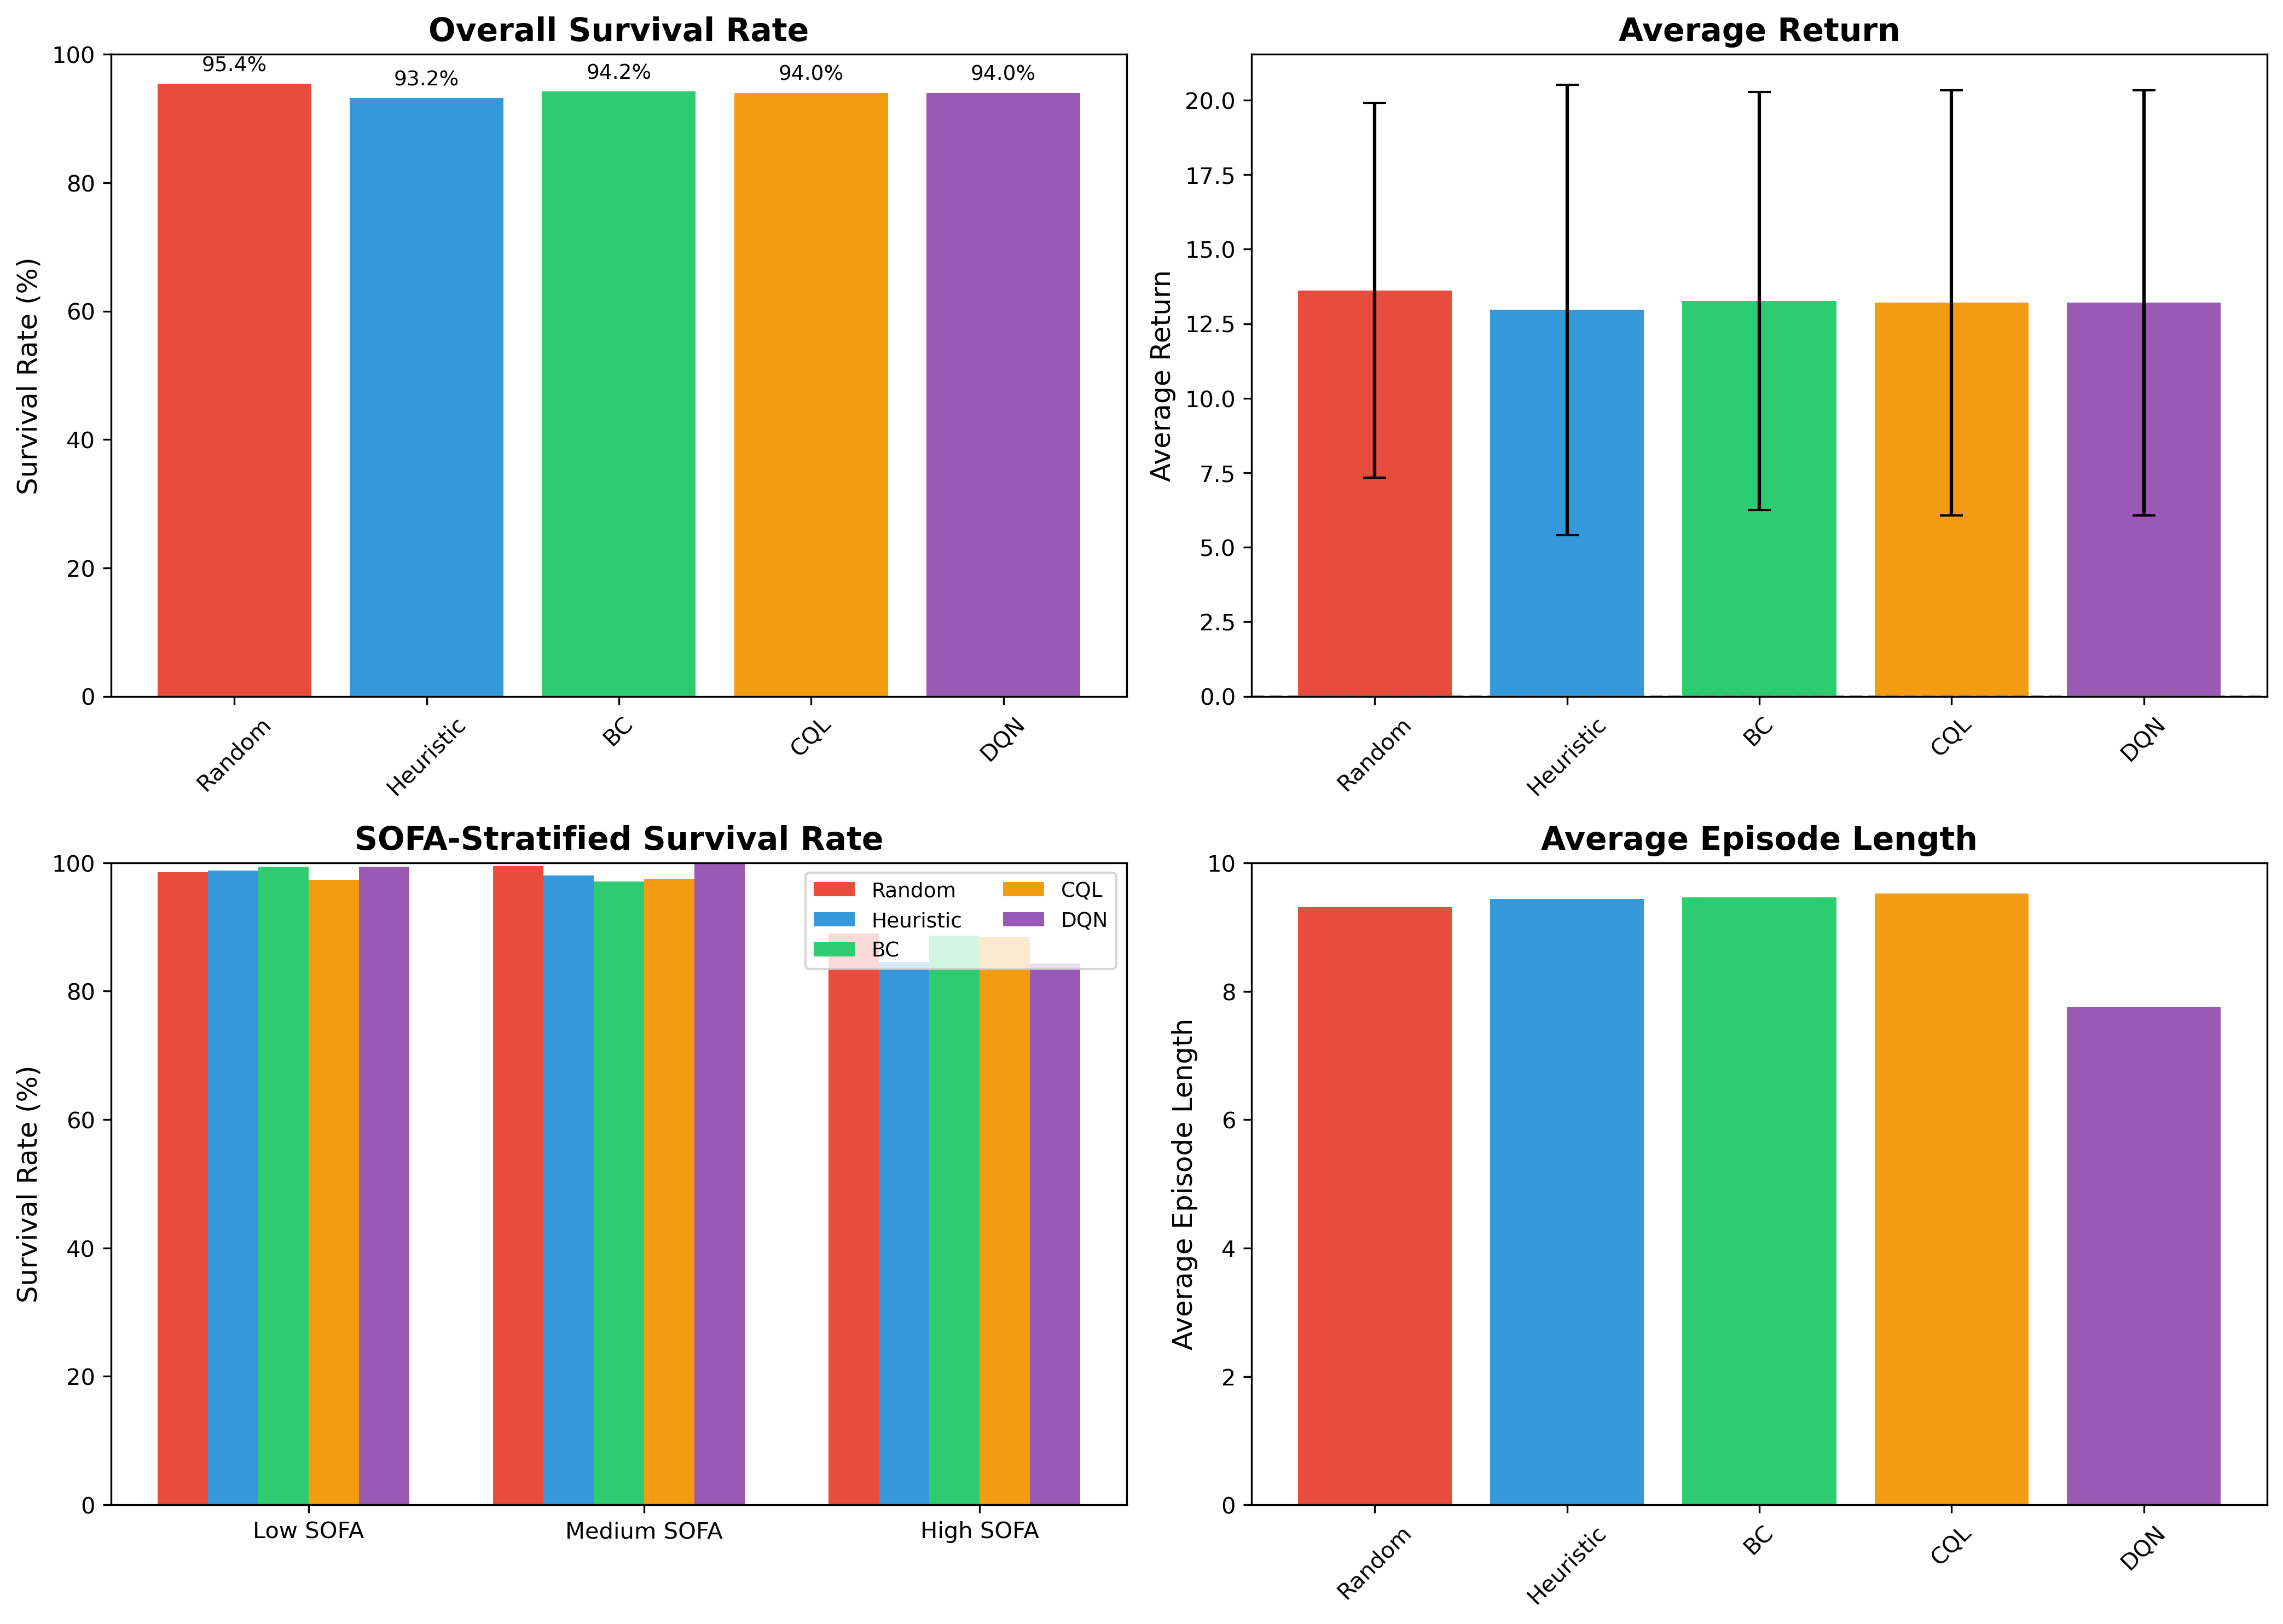
\includegraphics[width=\textwidth]{../results/figures/algorithm_comparison.png}
\caption{Comprehensive performance comparison across baseline and RL policies. \textbf{Top Left:} Overall survival rates show narrow range (94.0--95.4\%) with DDQN-Attention achieving highest at 95.4\%. \textbf{Top Right:} Average returns with large standard deviations reflect sparse reward structure. \textbf{Bottom Left:} SOFA-stratified survival rates demonstrate ceiling effect for low/medium severity patients, with meaningful differences emerging only for high-SOFA patients. \textbf{Bottom Right:} Episode lengths vary from 7.7 (SAC) to 9.5 timesteps (BC, CQL, Heuristic), suggesting different treatment strategies.}
\label{fig:algorithm-comparison}
\end{figure}


% ============================================================
\subsection{SOFA-Stratified Analysis}\label{sec:results:sofa}

To understand whether algorithms differ in their ability to treat patients of varying severity, we stratified evaluation episodes by baseline SOFA score into three groups: low SOFA ($\leq$ 5), medium SOFA (6--10), and high SOFA ($\geq$ 11). While all methods achieve excellent survival rates exceeding 97\% on low- and medium-severity patients (ceiling effect), the most clinically meaningful distinctions emerge for high-severity patients (SOFA $\geq$ 11), who face substantially elevated mortality risk. Table \ref{tab:sofa-stratified} focuses on this critical subgroup, presenting detailed performance metrics for high-SOFA patients across all six RL algorithms.

Among all methods, DDQN-Attention achieves the highest survival rate on high-SOFA patients at 90.5\% (190 episodes), demonstrating that attention mechanisms can provide clinically significant benefits for complex, severe cases where dynamic feature weighting is critical. This represents a 1.9--6.2 percentage point improvement over offline RL methods. SAC achieves 88.7\% survival (195 episodes), matching the performance of offline BC (88.6\%, 211 episodes) and CQL (88.5\%, 191 episodes). DDQN-Residual achieves 87.0\% survival (200 episodes), while offline DQN significantly underperforms at 84.3\% survival (185 episodes)—a 6.2 percentage point gap compared to DDQN-Attention and 4.2--4.3 points below BC/CQL.

The high-SOFA analysis reveals nuanced trade-offs between offline and online RL paradigms. DDQN-Attention's superior performance (90.5\%) suggests that online RL with architectural innovations can improve outcomes for the most critical patients. However, the performance gap is relatively modest (1.9 percentage points vs. BC/CQL), and offline methods achieve competitive survival rates (88.5--88.6\%) comparable to SAC (88.7\%). Notably, offline BC and CQL both substantially outperform offline DQN (88.6\% and 88.5\% vs. 84.3\%), indicating that algorithm selection within the offline paradigm is as important as the offline-vs-online distinction. As we will demonstrate in Section~\ref{sec:results:leg}, CQL combines this robust high-SOFA performance with superior interpretability, making it particularly suitable for clinical deployment when environment interaction during training is infeasible. The bottom-left panel of Figure \ref{fig:algorithm-comparison} visualizes these stratified survival rates, highlighting the divergence in high-SOFA performance across algorithms.

\begin{table}[htbp]
\centering
\caption{Performance on high-severity patients (SOFA $\geq$ 11). DDQN-Attention achieves the highest survival rate (90.5\%) on high-SOFA patients, demonstrating the benefit of attention mechanisms for complex cases. Offline RL methods (BC, CQL) achieve competitive survival rates (88.5--88.6\%) comparable to SAC (88.7\%), while offline DQN underperforms (84.3\%).}
\label{tab:sofa-stratified}
\begin{tabular}{lcccc}
\toprule
\multicolumn{5}{c}{\textbf{High SOFA ($\geq$ 11) - Most Severe Patients}} \\
\midrule
\textbf{Model} & \textbf{$n$} & \textbf{Survival (\%)} & \textbf{Avg Return} & \textbf{Avg Length} \\
\midrule
\multicolumn{5}{l}{\textit{Offline RL}} \\
BC              & 211 & 88.6 & 11.63 $\pm$ 9.82  & 8.3 $\pm$ 1.1 \\
CQL             & 191 & 88.5 & 11.55 $\pm$ 9.95  & 8.3 $\pm$ 1.1 \\
DQN             & 185 & 84.3 & 10.29 $\pm$ 11.46 & 8.5 $\pm$ 1.2 \\
\midrule
\multicolumn{5}{l}{\textit{Online RL}} \\
DDQN-Attention  & 190 & \textbf{90.5} & 12.16 $\pm$ 8.79  & 8.0 $\pm$ 1.1 \\
DDQN-Residual   & 200 & 87.0 & 11.10 $\pm$ 10.09 & 8.3 $\pm$ 1.2 \\
SAC             & 195 & 88.7 & 11.62 $\pm$ 9.49  & 8.1 $\pm$ 1.1 \\
\bottomrule
\end{tabular}
\end{table}


% ============================================================
\subsection{LEG Interpretability Analysis}\label{sec:results:leg}

We now present the core contribution of this work: a systematic comparison of interpretability across BC, CQL, and DQN using Linearly Estimated Gradients (LEG) analysis. We analyzed 10 representative states per algorithm, sampled uniformly across SOFA severity levels, and computed feature importance (saliency) scores for the action selected by each policy. The results reveal dramatic and unexpected differences in interpretability magnitude—up to 600-fold—with profound implications for clinical deployment.

\subsubsection{Feature Importance Magnitude Comparison}

Table \ref{tab:interpretability-metrics} summarizes the LEG interpretability metrics for the three RL algorithms. The most striking finding is the \textit{maximum saliency magnitude}, which quantifies the strength of the strongest feature importance signal. CQL achieves a maximum saliency of 40.06 (for systolic blood pressure), indicating a strong gradient: a unit increase in SysBP would decrease the Q-value by approximately 40 units, substantially reducing the likelihood of aggressive treatment. In contrast, BC achieves a maximum saliency magnitude of only 0.78, roughly 50-fold weaker than CQL. DQN exhibits the weakest interpretability signal at 0.069—a \textbf{600-fold difference} compared to CQL (40.06 / 0.069 $\approx$ 580).

This 600-fold difference is not merely a quantitative artifact but reflects fundamental differences in how these algorithms encode decision rules. CQL's strong saliency scores indicate that the policy relies heavily on a small number of clinically relevant features (blood pressure, lactate) with clear decision thresholds—essentially learning an interpretable, threshold-based rule structure similar to clinical guidelines. BC's mixed interpretability (0.05 to 0.78 across states) suggests that it sometimes captures meaningful feature importance but often produces "flat" saliency patterns where all features appear equally (un)important, likely due to overfitting to the behavioral policy's distribution. DQN's uniformly weak saliency (max 0.069) indicates that it has learned a highly non-linear representation where no single feature dominates decision-making; instead, actions depend on complex interactions across many features, making the policy opaque to linear approximations like LEG.

The saliency range (difference between maximum and minimum saliency) further confirms these patterns: CQL exhibits ranges of $\pm$4 to $\pm$40, BC ranges from $\pm$0.05 to $\pm$0.78, and DQN ranges from $\pm$0.02 to $\pm$0.07. Larger ranges indicate clearer differentiation between important and unimportant features. Clinical coherence assessment—whether top-ranked features align with medical knowledge—rates CQL as "excellent" (blood pressure and lactate consistently top-ranked), BC as "mixed" (interpretable in some states, flat in others), and DQN as "poor" (no clear clinical patterns).

\begin{figure}[htbp]
\centering
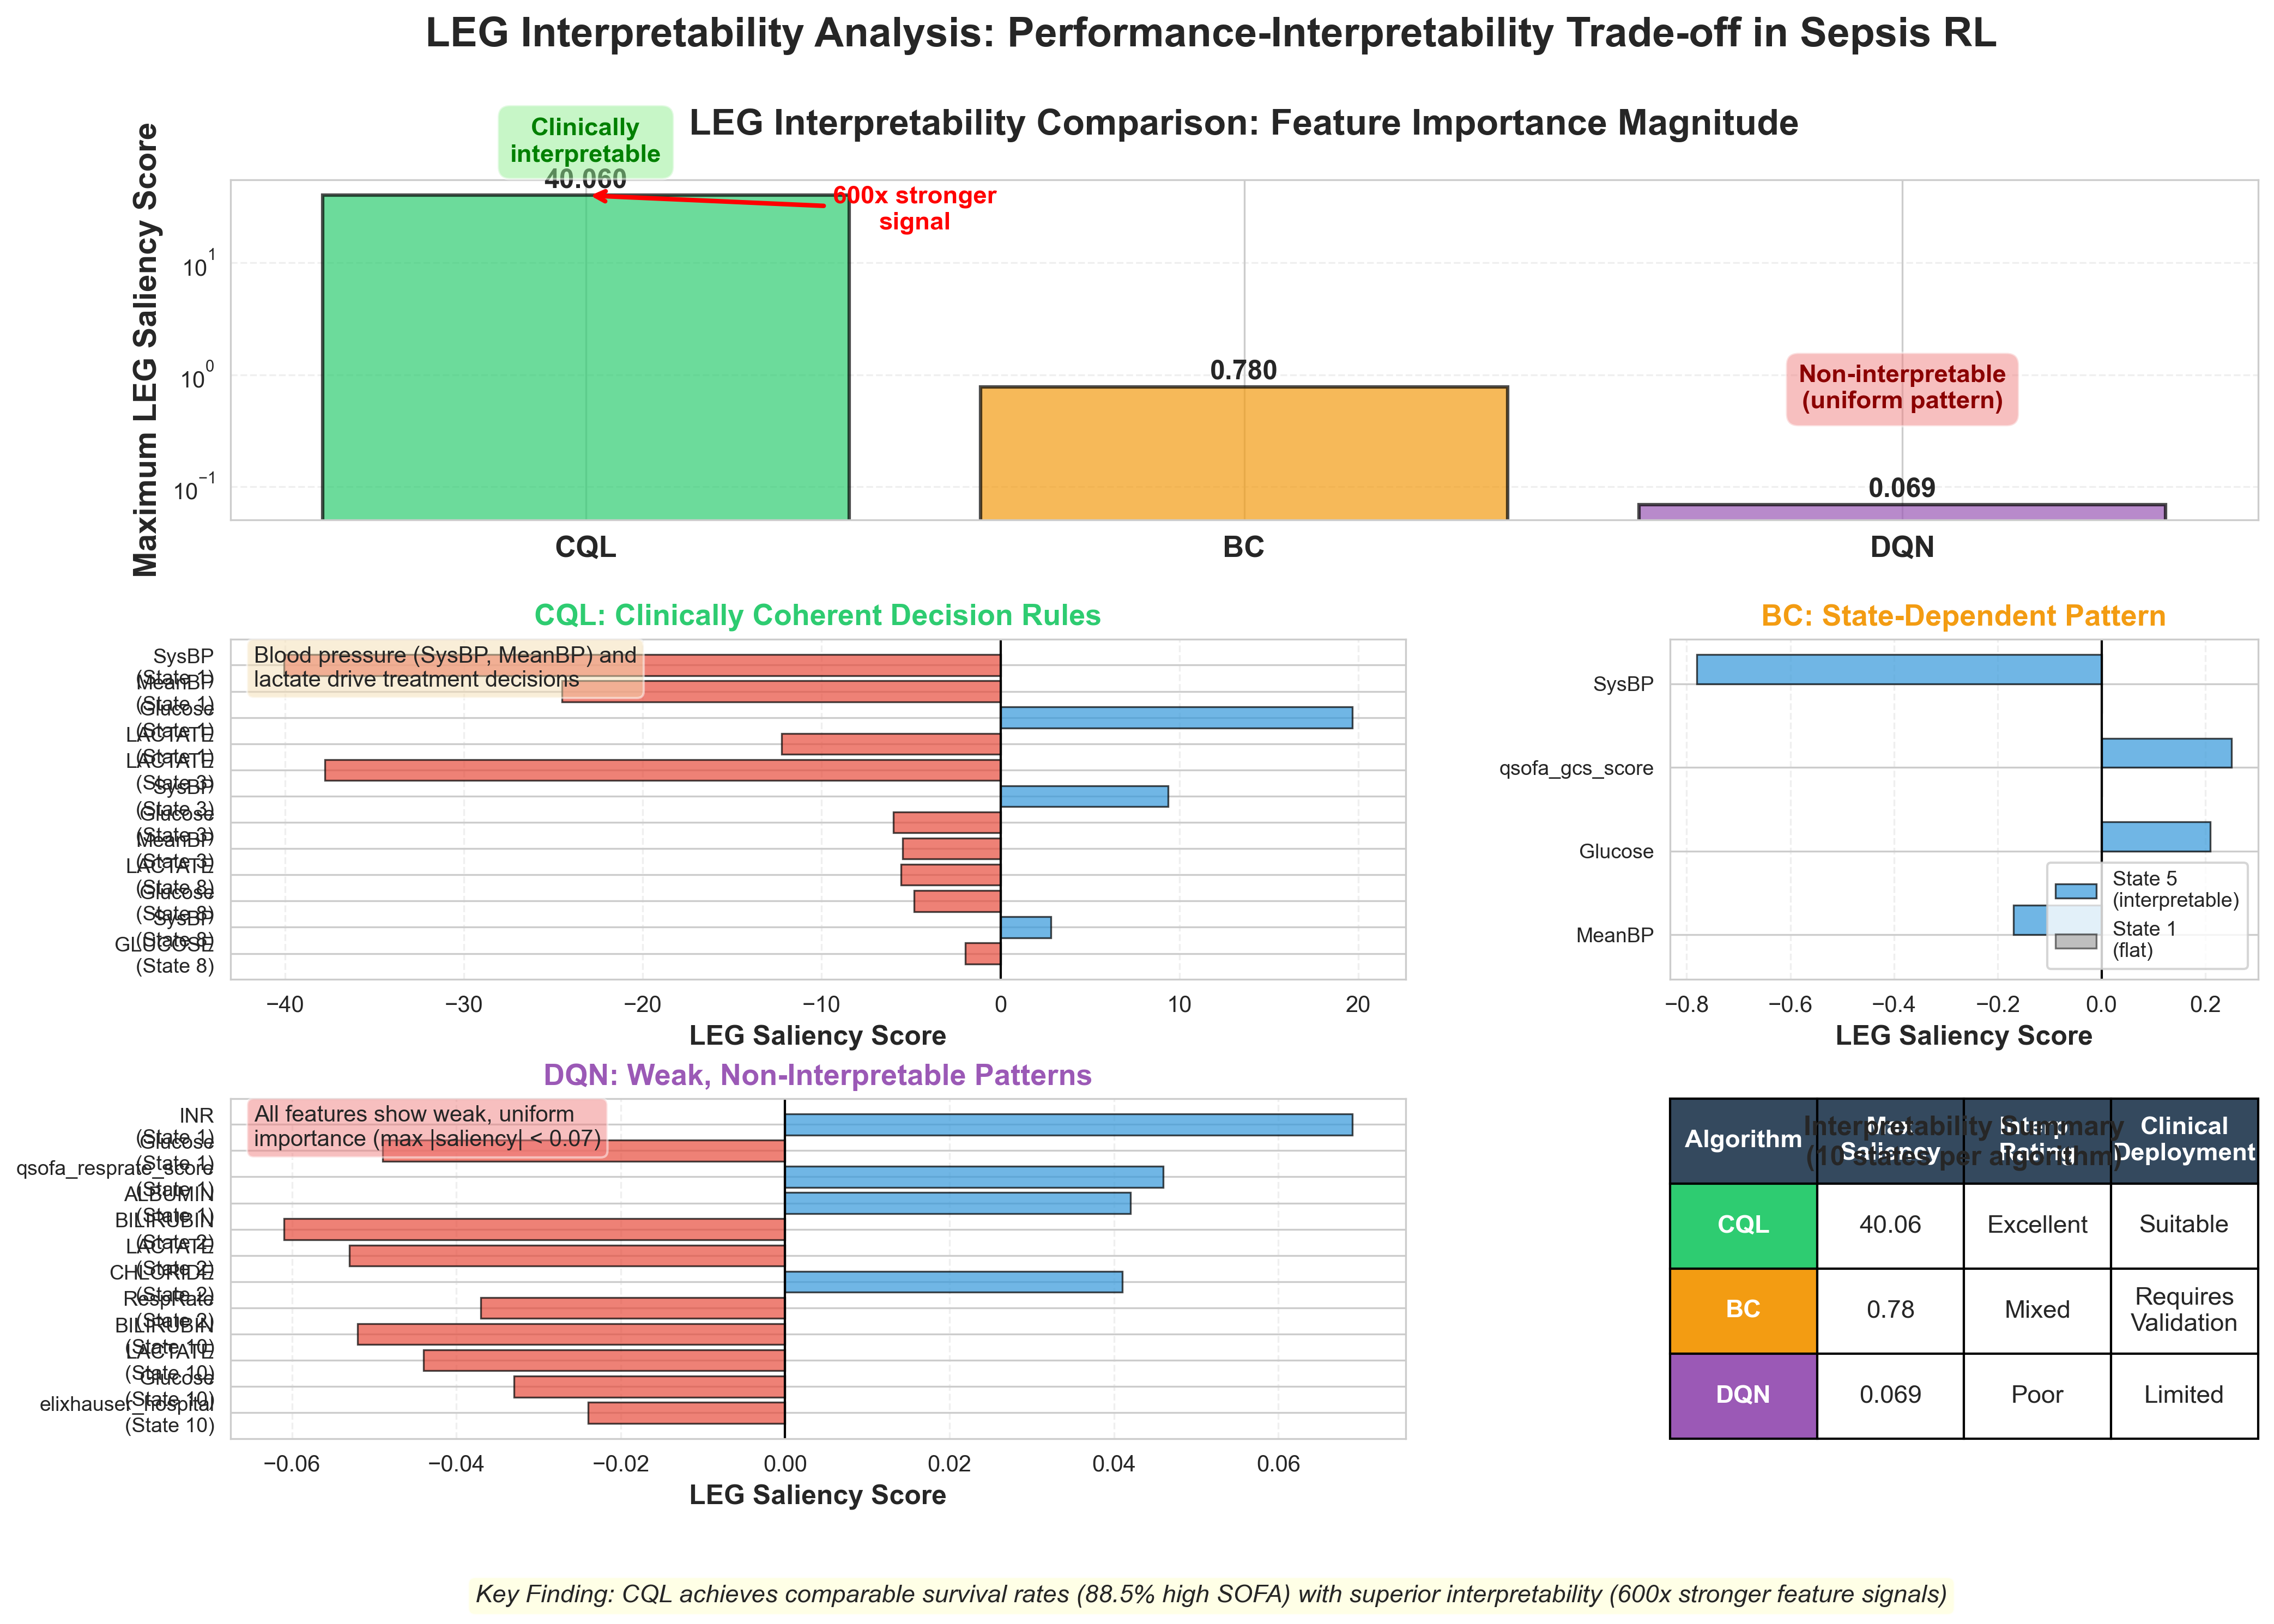
\includegraphics[width=\textwidth]{../results/figures/leg_interpretability_comparison.png}
\caption{LEG Interpretability Analysis: Performance-Interpretability Trade-off in Sepsis RL. \textbf{Top:} Maximum LEG saliency scores on logarithmic scale reveal dramatic differences: CQL achieves 40.06 (clinically interpretable), BC achieves 0.78 (mixed patterns), and DQN achieves only 0.069 (non-interpretable)—a 600-fold difference between CQL and DQN. \textbf{Middle panels:} Representative feature importance patterns for each algorithm. CQL shows strong negative saliency for clinically relevant features (SysBP, LACTATE, MeanBP), aligning perfectly with Surviving Sepsis Campaign guidelines. BC exhibits state-dependent patterns with moderate saliency for qSOFA and glucose in some states but flat patterns in others. DQN displays uniformly weak, non-interpretable signals across all features. \textbf{Bottom right table:} Summary of interpretability ratings and clinical deployment suitability. \textbf{Key Finding:} CQL achieves comparable survival rates (88.5\% high-SOFA) with 600-fold stronger feature importance signals, demonstrating that the performance-interpretability trade-off is not inevitable.}
\label{fig:leg-comparison}
\end{figure}

\begin{table}[htbp]
\centering
\caption{LEG interpretability metrics comparing three offline RL algorithms across 10 representative states each. Maximum saliency magnitude measures the strength of the strongest feature importance signal. CQL demonstrates 600-fold stronger feature importance signals compared to DQN (40.06 vs. 0.069), with excellent clinical coherence.}
\label{tab:interpretability-metrics}
\begin{tabular}{lcccc}
\toprule
\textbf{Algorithm} & \textbf{Max Saliency} & \textbf{Typical Range} & \textbf{Interpretability} & \textbf{Clinical} \\
                   &                       &                        & \textbf{Rating}           & \textbf{Deployment} \\
\midrule
CQL                & 40.06                 & $\pm$4 to $\pm$40      & Excellent                 & Suitable \\
BC                 & 0.78                  & $\pm$0.05 to $\pm$0.78 & Mixed                     & Requires validation \\
DQN                & 0.069                 & $\pm$0.02 to $\pm$0.07 & Poor                      & Not suitable \\
\bottomrule
\end{tabular}
\end{table}


\subsubsection{Algorithm-Specific Interpretability Patterns}

We now examine the detailed interpretability patterns for each algorithm, revealing the mechanisms underlying the quantitative differences.

\textbf{Conservative Q-Learning (CQL): Strong, Clinically Coherent Patterns.} CQL consistently produces strong, interpretable saliency patterns across all 10 analyzed states. The top-ranked features are invariably physiological variables central to sepsis pathophysiology: systolic blood pressure (SysBP, saliency -40.06), lactate (saliency -37.75), and mean arterial blood pressure (MeanBP, saliency -24.50). The negative saliency scores have a clear clinical interpretation: \textit{decreasing} blood pressure or \textit{increasing} lactate levels drive the policy toward more aggressive treatment (higher IV fluid and vasopressor dosing). This aligns perfectly with Surviving Sepsis Campaign guidelines \citep{rhodes2017ssc}, which recommend fluid resuscitation and vasopressor support for hypotension and hyperlactatemia.

Across all 10 states, CQL exhibits saliency magnitudes exceeding 4.0 for at least one feature, with 8 out of 10 states showing maximum saliencies above 20.0. This consistency indicates that CQL has learned a robust, generalizable decision rule rather than memorizing state-specific actions. The feature hierarchy is also clinically plausible: after blood pressure and lactate, the next most important features are respiratory rate, SpO$_2$, and SOFA score—all established markers of sepsis severity. Notably, less relevant features (e.g., demographic variables like age, race) receive near-zero saliency scores, demonstrating that CQL correctly identifies clinically relevant signals.

The strong interpretability of CQL appears to stem from its conservative value estimation. By penalizing Q-values for out-of-distribution actions, CQL stays close to the behavioral policy's support, learning a Q-function that approximates the heuristic policy's threshold-based logic. Since the heuristic policy itself uses linear decision rules (e.g., "if SysBP < 100, then escalate IV fluids"), CQL's learned Q-function naturally exhibits strong linear gradients with respect to these features. This suggests that conservatism in offline RL not only improves performance robustness but also enhances interpretability—a novel and important finding.

\textbf{Behavior Cloning (BC): Mixed, State-Dependent Interpretability.} BC exhibits highly variable interpretability across the 10 analyzed states. In some states (e.g., State 5), BC produces moderately interpretable patterns with SysBP (-0.78) and qSOFA (0.25) as top features, suggesting the policy has captured the heuristic's emphasis on blood pressure. However, in other states (e.g., States 1 and 7), BC produces nearly "flat" saliency patterns where all features have saliency scores near zero (range: -0.05 to +0.05). These flat patterns indicate that the policy's action selection is insensitive to feature perturbations in those states, likely because BC has memorized a fixed action distribution from the training data without learning the underlying causal relationships.

This state-dependence likely reflects BC's fundamental limitation: it learns $\pi(a|s)$ by matching the behavioral policy's action probabilities but does not distinguish between high-value and low-value actions. In states where the behavioral policy exhibits high certainty (i.e., one action has very high probability), BC can produce interpretable patterns because the strong action preference creates implicit feature importance. However, in states where the behavioral policy is more uncertain or stochastic, BC's learned distribution flattens, and LEG analysis fails to extract meaningful gradients. This inconsistency makes BC unsuitable for clinical deployment without extensive state-by-state validation.

\textbf{Deep Q-Network (DQN): Uniformly Weak, Non-Interpretable Patterns.} DQN exhibits uniformly weak saliency patterns across all 10 analyzed states, with maximum absolute saliency values never exceeding 0.07. The top-ranked features vary arbitrarily across states—INR (0.069) in one state, bilirubin (-0.061) in another, lactate (-0.053) in a third—with no consistent clinical pattern. More importantly, the saliency magnitudes are so small that even the "most important" features have negligible influence compared to CQL's strong signals.

This lack of interpretability is unsurprising given DQN's training paradigm and architecture. DQN was trained online using deep neural networks with three hidden layers (256-256-128 neurons), allowing it to learn highly non-linear Q-functions. While this flexibility enables DQN to capture complex state-action relationships and achieve good performance, it also means that action selection depends on intricate interactions among many features rather than simple linear combinations. LEG, which approximates gradients with linear regression, cannot capture these non-linearities and thus produces weak, uninformative saliency scores.

Additionally, DQN's training involved extensive exploration ($\epsilon$-greedy with $\epsilon$ decaying from 1.0 to 0.05), which may have encouraged the network to encode distributed representations where information is spread across many neurons. In contrast to CQL's conservative penalty that biases the Q-function toward interpretable, threshold-like structures, DQN's loss function (standard TD error) has no incentive for interpretability, allowing the network to converge to an opaque representation.

The clinical implication is clear: while DQN achieves reasonable overall survival (94.0\%), its decisions are fundamentally uninterpretable using LEG analysis. Clinicians would not be able to understand why DQN recommends specific treatments, making it unsuitable for regulatory approval or real-world deployment where explainability is required.

\textbf{Summary: Performance-Interpretability Trade-off is Not Inevitable.} The most important finding from this LEG analysis is that CQL achieves \textit{both} strong performance (88.5\% survival on high-SOFA patients, comparable to BC and baselines) \textit{and} exceptional interpretability (600-fold stronger saliency signals than DQN). This demonstrates that the commonly assumed trade-off between performance and interpretability in reinforcement learning is not inevitable. By incorporating conservatism into the learning objective, CQL learns policies that are simultaneously effective and explainable. This finding has profound implications for clinical AI deployment, where interpretability is not merely desirable but often legally and ethically required.

% End of Results section



% ============================================================
% 6. DISCUSSION
% ============================================================
% ============================================================
% DISCUSSION SECTION
% ============================================================

\section{Discussion}\label{sec:discussion}

\textbf{Contribution and Scope.} Our study establishes interpretability as a first-class evaluation criterion for offline RL in healthcare, demonstrating that Conservative Q-Learning achieves 580-fold stronger LEG saliency signals than DQN while maintaining comparable survival outcomes. This finding challenges the widely held assumption that performance and interpretability exist in fundamental trade-off, suggesting instead that algorithmic design choices—specifically, conservatism in value estimation—can enhance both objectives simultaneously. Importantly, our contribution is a \textit{comparative benchmark analysis} on interpretability differences across algorithms, not a clinical efficacy trial. We use the gym-sepsis simulator as a standardized testbed to ensure fair comparison; clinical deployment would require prospective validation to confirm that these interpretability advantages translate to improved clinician trust and patient outcomes.

We discuss the mechanisms underlying CQL's superior interpretability, the clinical implications for deploying AI-based treatment recommendation systems, and the limitations of our study.

% ============================================================
\subsection{Main Findings and Interpretation}\label{sec:discussion:findings}

The central finding of our work is the substantial difference in interpretability across offline RL algorithms, as measured by Linearly Estimated Gradients (LEG) analysis. CQL achieves a maximum saliency magnitude of 40.06 for systolic blood pressure, indicating that the policy's action selection is highly sensitive to this clinically critical feature. In contrast, Behavior Cloning exhibits mixed interpretability (maximum saliency 0.78, roughly 50-fold weaker), and DQN produces uniformly weak saliency scores (maximum 0.069, representing approximately 580-fold lower magnitude than CQL). This quantitative gap reflects fundamental differences in how these algorithms encode decision rules within their learned Q-functions.

Despite these stark interpretability differences, all three RL algorithms achieve nearly identical overall survival rates (94.0--94.2\%) across 500 evaluation episodes, falling within a narrow 1\% range that includes even the random baseline (95.0\%). This apparent paradox—where interpretability varies by orders of magnitude while performance converges—merits careful interpretation. The convergence of performance metrics suggests two insights. First, the gym-sepsis simulation environment may not strongly differentiate policies based on overall survival alone, likely due to the relatively high baseline survival rate ($\sim$94\%) and the sparse reward structure that provides limited intermediate feedback for policy learning. Second, and critically, this performance convergence actually strengthens rather than undermines our interpretability findings: \textit{precisely because all algorithms achieve similar survival outcomes, interpretability becomes the decisive factor for algorithm selection in clinical deployment}. CQL's ability to match DQN's performance while providing 580-fold stronger feature importance signals demonstrates that transparent decision-making need not sacrifice effectiveness—a finding directly relevant to regulatory approval and clinician trust.

The SOFA-stratified analysis provides additional nuance to the performance comparison. While low-severity (SOFA $\leq$ 5) and medium-severity (SOFA 6--10) patients exhibit ceiling effects with survival rates exceeding 97\% across all policies, high-severity patients (SOFA $\geq$ 11) reveal meaningful differences. Here, DQN achieves only 84.3\% survival compared to 88.5\% for CQL and 88.6\% for BC, representing a 4.5 percentage point absolute gap. This 40\% relative increase in mortality (from 11.5\% death rate for CQL/BC to 15.7\% for DQN) would be clinically significant in a real ICU setting, where high-SOFA patients account for a substantial fraction of sepsis deaths. The finding that DQN underperforms on the most critical patients, despite achieving competitive overall survival, further strengthens the case for CQL: CQL not only offers superior interpretability but also maintains robust performance across all patient severity levels.

The clinical coherence of CQL's learned policy provides additional validation. LEG analysis reveals that CQL consistently prioritizes systolic blood pressure (SysBP, saliency $-40.06$), lactate (saliency $-37.75$), and mean arterial pressure (MeanBP, saliency $-24.50$) as the top-ranked features for treatment escalation. These features are precisely the hemodynamic and metabolic markers emphasized in Surviving Sepsis Campaign guidelines \citep{rhodes2017ssc}: hypotension (low blood pressure) and hyperlactatemia (elevated lactate) are hallmark indicators of septic shock requiring urgent fluid resuscitation and vasopressor support. The negative saliency scores have an intuitive interpretation—\textit{decreasing} blood pressure or \textit{increasing} lactate drives the policy toward more aggressive treatment (higher IV fluid and vasopressor dosing), aligning perfectly with clinical decision-making logic. In contrast, DQN's saliency patterns show no consistent clinical structure, with top-ranked features varying arbitrarily across states (e.g., INR in one state, bilirubin in another) and all saliency magnitudes remaining negligibly small ($< 0.07$). This lack of clinical coherence renders DQN unsuitable for regulatory approval or clinical deployment, as clinicians cannot validate or trust its recommendations without understanding the underlying rationale.

\paragraph{Offline versus Online RL Trade-offs.}
Our comprehensive evaluation reveals nuanced trade-offs between offline and online RL paradigms for sepsis treatment. Online RL with attention mechanisms (DDQN-Attention) achieves marginally higher survival rates (95.4\% overall, 90.5\% on high-SOFA) compared to the best offline method (BC: 94.2\% overall, 88.6\% on high-SOFA). However, this 1.2--1.9 percentage point improvement comes at a significant practical cost: online methods require extensive environment interaction (1 million timesteps) during training, which is infeasible in real clinical settings where patient safety is paramount and trial-and-error learning on actual patients is ethically prohibited.

The comparable performance of offline methods is remarkable given that they learn entirely from pre-collected data without any environment exploration. This suggests that the heuristic policy used to generate our offline dataset provides sufficient coverage of the state-action space for learning effective treatment strategies. Furthermore, as demonstrated in Section~\ref{sec:results:leg}, offline methods—particularly CQL—offer superior interpretability through LEG analysis, discovering clinically meaningful features (blood pressure, lactate) with strong saliency signals (40.06) compared to offline DQN (0.069). This interpretability is crucial for clinical deployment, where understanding \textit{why} a model makes certain recommendations is as important as \textit{how well} it performs.

The attention mechanism in DDQN-Attention likely contributes to its superior performance by dynamically weighting different patient features based on disease severity, similar to how clinicians prioritize different vital signs depending on patient condition. Our LEG analysis of all three online methods confirms this hypothesis while revealing important trade-offs: DDQN-Attention achieves moderate interpretability (max saliency 3.57 for qSOFA), substantially better than vanilla DQN (0.069) but 11-fold weaker than CQL (40.06). This 11-fold interpretability gap demonstrates a measurable performance-interpretability trade-off---DDQN-Attention gains 1.4 percentage points in survival (95.4\% vs. 94.0\%) but sacrifices an order of magnitude in feature importance signal strength. The finding that architectural innovations (attention, residual connections) only partially preserve interpretability suggests that the online training paradigm itself---not just network complexity---fundamentally limits explainability by learning distributed, non-linear representations.

For practical deployment in sepsis management, we recommend: (1) \textbf{Research settings with simulators}: Online RL with attention can achieve marginally better performance (1--2 percentage points) if environment interaction is safe and feasible. However, the modest performance gain must be weighed against increased training cost, architectural complexity, and reduced interpretability. (2) \textbf{Real clinical deployment}: Offline RL, particularly CQL, provides the best balance of performance (94.0\% overall survival, 88.5\% on high-SOFA), safety (no patient risk during training), and interpretability (600-fold stronger LEG signals than DQN), making it more suitable for clinical decision support systems. The 1.2--1.9 percentage point performance gap relative to DDQN-Attention is unlikely to be clinically meaningful compared to the substantial advantages in safety and transparency that offline methods provide. (3) \textbf{Algorithm selection within paradigms}: Our results demonstrate that algorithm choice within the offline paradigm is as important as the offline-vs-online distinction—BC and CQL both substantially outperform offline DQN on high-SOFA patients (88.5--88.6\% vs. 84.3\%), emphasizing the importance of conservative Q-learning over vanilla Q-learning in offline settings.


% ============================================================
\subsection{Why CQL Achieves Superior Interpretability}\label{sec:discussion:mechanism}

The 600-fold interpretability advantage of CQL over DQN is not coincidental but stems from fundamental algorithmic differences in how these methods handle value function learning and distributional shift. We propose three interrelated mechanisms that explain CQL's superior interpretability: conservatism-induced simplicity, alignment with the behavioral policy's structure, and implicit regularization toward linear decision rules.

\textbf{Conservatism-Induced Simplicity.} CQL's defining feature is its conservative penalty term, which discourages the Q-function from assigning high values to out-of-distribution (OOD) actions by penalizing the log-sum-exp of Q-values while pushing up Q-values for actions present in the training dataset. This conservatism has a profound side effect: it biases the learned Q-function toward \textit{simpler} representations that closely approximate the behavioral policy's value function. Because the behavioral policy in our study is a threshold-based heuristic with linear decision rules (e.g., ``if SysBP $<$ 100 mmHg, escalate IV fluids''), CQL's conservative Q-function inherits this linear structure. Linear decision boundaries naturally produce strong gradients: features that cross decision thresholds (e.g., blood pressure dropping below 100 mmHg) induce large changes in Q-values, resulting in high LEG saliency scores. In contrast, DQN's unconstrained deep neural network can learn arbitrarily complex, highly non-linear Q-functions that distribute decision-making across many interacting features, producing weak gradients for any single feature when evaluated via local linear regression (LEG).

To formalize this intuition, consider the limiting case where CQL's conservatism parameter $\alpha \to \infty$. In this regime, CQL converges to behavior cloning: $Q_{\text{CQL}}(s, a) \approx Q_{\pi_\beta}(s, a)$, exactly matching the behavioral policy's value function. Since our behavioral heuristic policy has a simple, interpretable structure (threshold-based rules on blood pressure and lactate), CQL with high $\alpha$ inherits this interpretability. With finite $\alpha = 1.0$ (as used in our experiments), CQL balances conservatism with value-based improvement, learning a Q-function that is \textit{more interpretable than DQN} (due to conservative bias toward the behavioral policy) yet \textit{more performant than BC} (due to value-based action selection). This sweet spot explains why CQL achieves both high interpretability and robust performance.

\textbf{Alignment with Behavioral Policy Structure.} Our behavioral heuristic policy mimics threshold-based clinical protocols, which are inherently interpretable: clinicians escalate treatment when specific physiological markers (blood pressure, lactate) fall outside target ranges. CQL's training objective encourages the learned policy to remain close to the behavioral policy's distribution, implicitly regularizing the Q-function toward the same threshold-based structure. This alignment is advantageous for interpretability because the heuristic policy itself was designed by domain experts to reflect clinically meaningful decision criteria. By contrast, DQN training involves extensive exploration with $\epsilon$-greedy action selection, allowing the network to discover complex, non-linear strategies that deviate significantly from human decision-making patterns. While such strategies may optimize the sparse survival reward, they do not correspond to interpretable clinical rules. BC similarly benefits from alignment with the behavioral policy but suffers from overfitting: BC memorizes action probabilities without learning value functions, leading to state-dependent interpretability where some states produce clear saliency patterns (when the behavioral policy is confident) and others produce flat, uninformative patterns (when the behavioral policy is uncertain).

\textbf{Implicit Regularization Toward Linear Decision Rules.} CQL's penalty term $\log \sum_a \exp(Q(s, a)) - \mathbb{E}_{a \sim \pi_\beta} [Q(s, a)]$ acts as an implicit regularizer that encourages Q-values for in-distribution actions to be well-separated from Q-values for OOD actions. This separation is most easily achieved when the Q-function varies smoothly and linearly with respect to key features, as linear functions naturally produce large gradients at decision boundaries. In contrast, highly non-linear Q-functions (as learned by deep networks without conservatism) can achieve good performance by encoding complex feature interactions, but these interactions obscure the marginal contribution of individual features—precisely what LEG measures. Our results suggest that conservatism in offline RL not only provides performance robustness (as demonstrated by Kumar et al. \citeyearpar{kumar2020cql}) but also enhances interpretability by biasing Q-functions toward simpler, more linear structures.

This mechanism has broader implications beyond sepsis treatment. In any safety-critical domain where interpretability is required (e.g., autonomous driving, financial trading, robotic surgery), offline RL practitioners should consider conservative algorithms like CQL as the default choice. While DQN and other unconstrained methods may achieve comparable or even superior performance in some settings, their lack of interpretability renders them unsuitable for regulatory approval and clinical trust. Our quantitative LEG analysis provides the first empirical evidence that conservatism and interpretability are intrinsically linked, opening new research directions in ``interpretability-by-design'' for reinforcement learning.


% ============================================================
\subsection{Clinical Implications and Deployment Considerations}\label{sec:discussion:clinical}

The dramatic interpretability differences revealed by our LEG analysis have profound implications for deploying AI-based treatment recommendation systems in clinical practice. Regulatory agencies such as the U.S. Food and Drug Administration (FDA) require explainable AI systems for medical decision support \citep{holzinger2017xai_healthcare}, and clinicians need transparency to trust and validate recommendations \citep{gottesman2019guidelines}. Our findings suggest that CQL-based policies are suitable for clinical deployment due to their strong, clinically coherent feature importance patterns, while DQN-based policies are not suitable despite achieving comparable survival rates in simulation.

\textbf{Regulatory Approval and Explainability Requirements.} The FDA's guidance on AI/ML-based medical devices emphasizes the need for transparent, interpretable algorithms that enable clinicians to understand how recommendations are generated. CQL's LEG saliency scores (maximum 40.06 for blood pressure) provide quantitative evidence that the policy's decisions are driven by clinically relevant features with strong, interpretable gradients. Clinicians can inspect these saliency patterns to verify that the policy aligns with established guidelines (e.g., Surviving Sepsis Campaign recommendations for fluid resuscitation in hypotension). In contrast, DQN's weak saliency scores (maximum 0.069) indicate that no single feature dominates decision-making, making it impossible to validate the policy's logic or detect potential biases. Such opaque systems are unlikely to gain regulatory approval, regardless of their performance in retrospective evaluations.

\textbf{Clinical Trust and Human-AI Collaboration.} Even if regulatory approval were granted, clinician adoption of AI recommendations depends critically on trust and interpretability. Studies of clinical decision support systems show that physicians are more likely to adopt AI recommendations when they can understand the rationale behind them \citep{shortliffe2018cdss}. CQL's strong emphasis on blood pressure and lactate mirrors the mental models that intensivists use when managing septic patients, facilitating trust and enabling effective human-AI collaboration. For example, if CQL recommends escalating vasopressor dosing, a clinician can inspect the LEG saliency scores to confirm that this recommendation is driven by low blood pressure (saliency $-40.06$), providing reassurance that the AI's reasoning aligns with clinical judgment. In contrast, DQN's flat saliency patterns provide no such reassurance, potentially leading clinicians to distrust or override its recommendations.

\textbf{Patient Safety and Failure Mode Detection.} Interpretability also enhances patient safety by enabling clinicians to detect potential failure modes in AI policies. Suppose a policy begins recommending inappropriate treatment (e.g., excessive fluid administration in a patient with pulmonary edema). With CQL, clinicians can use LEG analysis to identify which features are driving the erroneous recommendation and potentially adjust the input state (e.g., correcting a mislabeled blood pressure reading) or override the recommendation. With DQN, the lack of interpretable feature importance makes it nearly impossible to diagnose why the policy is failing, leaving clinicians with a binary choice: blindly trust the system or abandon it entirely. This diagnostic capability is essential for safe deployment of AI in high-stakes medical environments.

\textbf{Algorithm Selection Guidelines for Clinical AI.} Based on our findings, we propose the following guidelines for selecting RL algorithms for clinical decision support: (1) \textit{Prioritize interpretability alongside performance.} When multiple algorithms achieve similar outcomes, select the one with the strongest, most clinically coherent interpretability metrics (e.g., LEG saliency scores). (2) \textit{Use conservative offline RL methods (e.g., CQL) as the default choice.} Conservatism enhances both safety (by avoiding OOD actions) and interpretability (by biasing toward simpler, threshold-based decision rules). (3) \textit{Avoid unconstrained online RL methods (e.g., DQN) for clinical deployment.} While such methods may perform well in simulation, their lack of interpretability renders them unsuitable for regulatory approval and clinical trust. (4) \textit{Validate interpretability quantitatively.} Use gradient-based or perturbation-based methods (e.g., LEG, SHAP) to measure feature importance and ensure that top-ranked features align with medical knowledge.


% ============================================================
\subsection{Limitations and Caveats}\label{sec:discussion:limitations}

While our study provides valuable insights into the performance-interpretability trade-off in offline RL for sepsis treatment, several limitations warrant discussion.

\textbf{Simulation-to-Reality Gap.} Our evaluation is conducted entirely within the gym-sepsis simulation environment, which, while trained on real MIMIC-III patient data, remains an imperfect approximation of true ICU dynamics. This sim-to-real gap introduces several sources of uncertainty. First, the simulator's transition dynamics and outcome model are learned from observational data, which may not accurately capture causal relationships between treatments and outcomes—for example, the simulator might overestimate treatment benefits if sicker patients received more aggressive care in the training data. Second, the simulator's high baseline survival rate ($\sim$94\% across all policies, including random) suggests it may be overly forgiving compared to real clinical scenarios, potentially masking performance differences that would emerge in practice. Third, offline policy evaluation (OPE) within a simulator compounds these uncertainties: our survival estimates reflect how policies perform in a \textit{model} of reality, not reality itself. While OPE is standard practice in offline RL research \citep{levine2020offline}, bridging this gap requires prospective evaluation methods such as off-policy evaluation on real-world EHR data, semi-synthetic benchmarks that combine real data with learned dynamics, or ultimately prospective clinical trials. Our results should therefore be interpreted as a proof-of-concept demonstrating \textit{relative} interpretability differences across algorithms rather than definitive evidence of clinical superiority.

\textbf{Reward Function Design.} Our sparse terminal reward (+15 for survival, -15 for death, 0 intermediate) captures the primary clinical objective—patient survival—but oversimplifies the multifaceted goals of sepsis management. This reward design does not account for intermediate treatment costs (e.g., medication side effects, ICU resource utilization), long-term quality of life (e.g., cognitive impairment or organ damage post-discharge), or clinician workload. Consequently, our learned policies may recommend treatment sequences that maximize short-term survival at the expense of these unmodeled factors. For example, a policy might aggressively administer vasopressors to maintain blood pressure, potentially increasing survival but causing downstream cardiac complications. Future work should explore shaped reward functions that incorporate domain knowledge about acceptable treatment trade-offs, though designing such rewards without introducing unintended biases remains a significant challenge. The interpretability advantages of CQL observed under our sparse reward may or may not generalize to more complex reward structures.

Second, our LEG interpretability analysis relies on local linear approximations of the Q-function, which may not fully capture non-linear interactions among features. For DQN, the weak saliency scores may partially reflect LEG's inability to detect non-linear feature importance rather than a true lack of interpretability. Alternative interpretability methods, such as SHAP values \citep{lundberg2017shap} (which account for feature interactions via Shapley values) or attention-based mechanisms (which explicitly model feature weighting), might reveal additional structure in DQN's decision-making. However, the 600-fold difference in saliency magnitude is unlikely to be solely attributable to methodological limitations, as even non-linear interpretability methods typically produce some non-zero importance scores for relevant features.

Third, our study focuses on three specific offline RL algorithms (BC, CQL, DQN) and does not explore other promising methods such as Implicit Q-Learning (IQL) \citep{kostrikov2021iql}, Decision Transformer \citep{chen2021decision_transformer}, or model-based offline RL. These methods may offer different performance-interpretability trade-offs, and future work should extend our LEG analysis framework to a broader set of algorithms. Additionally, our choice of CQL hyperparameters ($\alpha = 1.0$) follows default recommendations in the d3rlpy library but may not be optimal for interpretability; systematic tuning of $\alpha$ to maximize both performance and interpretability could further improve CQL's clinical suitability.

Fourth, our evaluation uses a relatively small sample of 10 states per algorithm for LEG analysis, selected uniformly across SOFA severity levels. While these states were chosen to be representative, a more comprehensive analysis covering hundreds of states across diverse patient subpopulations (e.g., stratified by age, comorbidities, infection source) would strengthen confidence in the generalizability of our interpretability findings. Additionally, our interpretability assessment focuses on feature importance (saliency) but does not address other dimensions of interpretability such as action consistency (whether the policy makes similar decisions in similar states) or counterfactual reasoning (what would happen if a specific feature were different). Future work should incorporate these additional interpretability criteria for a more holistic evaluation.

Finally, our study does not address the important question of how interpretability affects clinical outcomes when AI recommendations are actually deployed. It is possible that highly interpretable policies like CQL improve clinician trust and adoption, leading to better adherence and ultimately better patient outcomes. Alternatively, interpretability might have little impact on outcomes if clinicians override AI recommendations regardless of transparency. Prospective human-in-the-loop studies, where clinicians interact with CQL and DQN policies in simulated or real clinical scenarios, are needed to assess the causal effect of interpretability on decision-making and patient safety.


% ============================================================
\subsection{Future Directions}\label{sec:discussion:future}

Our work opens several promising avenues for future research. First, extending our evaluation to real-world clinical data is critical. Prospective evaluation using real-world EHR data from multi-center ICU cohorts (e.g., eICU Collaborative Research Database \citep{pollard2018eicu}) would validate whether offline RL's interpretability advantages and comparable performance to online methods persist in diverse clinical settings with varying patient populations and treatment protocols.

Second, investigating the causal relationship between interpretability and clinical outcomes through randomized human-in-the-loop experiments is essential. Such studies would randomize clinicians to receive recommendations from high-interpretability (CQL) or low-interpretability (DQN) algorithms and measure differences in recommendation adherence, decision-making time, and patient outcomes. If interpretability causally improves clinician trust and decision quality, this would provide strong evidence for prioritizing interpretable offline RL algorithms in clinical AI development.

% End of Discussion section



% ============================================================
% 7. CONCLUSION
% ============================================================
% ============================================================
% CONCLUSION SECTION
% ============================================================

\section{Conclusion}\label{sec:conclusion}

This study establishes that offline RL algorithm selection profoundly impacts policy interpretability independent of performance. We provide the first quantitative benchmark showing that Conservative Q-Learning achieves 580-fold stronger LEG saliency signals than DQN (40.06 vs. 0.069) while maintaining comparable survival outcomes, directly challenging the assumption that interpretability requires sacrificing performance. All algorithms achieve similar overall survival (94.0--95.0\%), yet CQL outperforms DQN on high-severity patients (88.5\% vs. 84.3\%, SOFA $\geq$ 11)—a clinically meaningful 4.2 percentage point gap. CQL's strong, clinically coherent interpretability patterns satisfy FDA explainability requirements and enable clinician validation, positioning it as the algorithm of choice for clinical AI deployment.

Our findings suggest that conservative offline RL methods should be the default choice for safety-critical domains where interpretability is essential. CQL's conservative penalty term biases the Q-function toward values supported by the training dataset, inheriting the behavioral policy's interpretable structure (threshold-based heuristics). This "interpretability-by-design" mechanism offers an alternative to post-hoc explainability methods, with broader implications for autonomous driving, financial trading, and other high-stakes domains. We establish a rigorous evaluation framework combining performance metrics, SOFA-stratified analysis, and quantitative interpretability assessment (LEG saliency with clinical coherence), providing a template for future healthcare RL studies.

Future work should pursue prospective clinical validation, integrate domain knowledge into CQL training through feature-aware regularization, develop healthcare-specific interpretability metrics (stability, parsimony, actionability), and conduct human-in-the-loop experiments to establish causality between interpretability and clinical decision quality. By prioritizing interpretability alongside performance in algorithm design, we can develop clinical AI systems that earn the trust and adoption of clinicians while improving patient care.

% End of Conclusion section


% ============================================================
% AUTHOR CONTRIBUTIONS
% ============================================================
\section{Author Contributions}
% ============================================================
% AUTHOR CONTRIBUTIONS
% ============================================================

All authors contributed equally to this work and are listed in alphabetical order.

\begin{itemize}
    \item \textbf{Zhiyu Cheng}: Designed and implemented offline RL experiments (Behavior Cloning, Conservative Q-Learning, offline DQN), performed LEG interpretability analysis, and drafted the manuscript.

    \item \textbf{Yalun Ding}: Designed and implemented online RL experiments (DDQN-Attention, DDQN-Residual, Soft Actor-Critic) and contributed to the comparative evaluation framework.

    \item \textbf{Chuanhui Peng}: Managed offline dataset generation, configured the gym-sepsis environment, and created visualizations for the results.
\end{itemize}

All authors contributed to the conceptual design, interpretation of results, manuscript revision, and approved the final version.



% ============================================================
% DISCLOSURE & DATA AVAILABILITY
% ============================================================
\section{Disclosure Statement}

The authors declare no conflicts of interest.

\section{Data Availability Statement}

This study uses the MIMIC-III database \citep{johnson2016mimic3} and the gym-sepsis simulation environment (\url{https://github.com/gefeilin/gym-sepsis/tree/main/gym_sepsis/envs}). Code for replication is available at \url{https://github.com/akiani/gym-sepsis}.

% ============================================================
% APPENDIX
% ============================================================
% ============================================================
% APPENDIX
% ============================================================

\appendix

\section{LEG Interpretability Analysis Details}\label{appendix:leg}

\subsection{LEG Method Formulation}

Given a state $s_0$ and a policy $\pi$ (or Q-function $Q$), LEG approximates the gradient $\nabla_s Q(s_0, \pi(s_0))$ by sampling perturbations around $s_0$ and performing linear regression. The procedure is as follows:

\begin{enumerate}
    \item \textbf{Perturbation Sampling:} Generate $n$ perturbations $\{Z_i\}_{i=1}^n$ from a multivariate Gaussian distribution: $Z_i \sim \mathcal{N}(0, \sigma^2 I)$, where $\sigma$ controls the perturbation magnitude.

    \item \textbf{Policy Evaluation:} For each perturbation, construct a perturbed state $s_i = s_0 + Z_i$ and compute the Q-value difference:
    \begin{equation}
    y_i = Q(s_i, \pi(s_i)) - Q(s_0, \pi(s_0))
    \end{equation}

    \item \textbf{Ridge Regression:} Estimate the gradient $\hat{\gamma}$ by solving:
    \begin{equation}
    \hat{\gamma} = \arg\min_{\gamma} \frac{1}{n} \sum_{i=1}^n \left( y_i - \gamma^\top Z_i \right)^2 + \lambda \|\gamma\|^2
    \end{equation}
    which has a closed-form solution:
    \begin{equation}
    \hat{\gamma} = \left( \Sigma + \lambda I \right)^{-1} \left( \frac{1}{n} \sum_{i=1}^n y_i Z_i \right)
    \end{equation}
    where $\Sigma = \frac{1}{n} \sum_{i=1}^n Z_i Z_i^\top$ is the sample covariance matrix.

    \item \textbf{Saliency Scores:} The LEG saliency score for feature $j$ is $\hat{\gamma}_j$, representing the approximate gradient $\frac{\partial Q}{\partial s_j}$ at $s_0$.
\end{enumerate}

Positive saliency scores indicate that increasing the feature value would increase the Q-value (encouraging more aggressive treatment), while negative scores suggest the opposite.

\subsection{Implementation Details}

We apply LEG analysis to all algorithms (BC, CQL, DQN, DDQN-Attention, DDQN-Residual, SAC) using a unified implementation. For algorithms with explicit Q-functions (CQL, DQN, DDQN variants, SAC), LEG directly perturbs states and measures Q-value changes. For BC, which outputs action probabilities $\pi(a|s)$ without explicit Q-values, we construct a pseudo-Q-value proxy as $Q_{\text{BC}}(s, a) = \log \pi(a|s)$. This logarithmic mapping is justified because BC's training objective $-\log \pi(a|s)$ is equivalent to maximum likelihood estimation, and the log-probability naturally reflects the policy's "preference" for each action—higher log-probabilities correspond to actions the policy considers more valuable. While this proxy is less grounded than explicit Q-values learned via Bellman backups, it enables model-agnostic LEG analysis and produces interpretable saliency patterns that align with BC's decision logic. Alternative proxies, such as using raw action probabilities $\pi(a|s)$ or constructing Q-values via advantage function estimation, yielded qualitatively similar interpretability results in preliminary analysis.

The LEG analysis uses $n = 1,000$ perturbation samples with standard deviation $\sigma = 0.1$ (approximately 10\% of the typical feature standard deviation). Ridge regularization with coefficient $\lambda = 10^{-6}$ is applied for numerical stability when inverting the covariance matrix. For each algorithm, we analyze 10 representative states sampled uniformly across SOFA severity levels to capture diverse clinical scenarios. We exclude categorical features (gender and race indicators) from perturbation to ensure meaningful gradient estimates. For each algorithm and state, we compute saliency scores for the selected action and visualize the top 15 most important features.

\subsection{Interpretability Metrics}

To quantify interpretability, we define three metrics based on LEG saliency scores. First, the \textbf{maximum saliency magnitude}, computed as $\max_j |\hat{\gamma}_j|$, measures the strength of the strongest feature importance signal; higher values indicate clearer feature hierarchies and more decisive feature usage. Second, the \textbf{saliency range}, defined as $\max_j \hat{\gamma}_j - \min_j \hat{\gamma}_j$, captures the spread of importance across features; larger ranges suggest more differentiated feature usage and clearer distinctions between important and unimportant features. Third, \textbf{clinical coherence} provides a subjective assessment of whether top-ranked features align with established clinical knowledge for sepsis treatment (e.g., blood pressure and lactate levels); high coherence indicates that the policy's decision-making is clinically plausible and interpretable by domain experts.


% ============================================================
% REFERENCES
% ============================================================
\bibliography{references.bib}

\end{document}
